\documentclass[article]{uom-coursework}
\usepackage[showframe]{geometry}

\usetikzlibrary{automata, positioning, arrows,
arrows.meta}

\usepackage{float}
\usepackage{syntax}
\usepackage{mdframed}
\usepackage[ruled]{algorithm2e}
\usepackage[nopagecolor={white}]{pagecolor}
% \usepackage{contour}
\usepackage{soul}
\usepackage{calc}
% \usepackage[normalem]{ulem}
% \usepackage[luatex]{accsupp}


% \setlength{\ULdepth}{1.8pt}
% \contourlength{1pt}

% \newcommand{\ul}[1]{
% \BeginAccSupp{method=plain,ActualText={#1}}%
% \uline{\hphantom{#1}}%
% % \llap{\contour{\thepagecolor}{#1}}%
% \EndAccSupp{}%
% }

% \newcommand{\ul}[1]{
% \uline{\hphantom{#1}}%
% \llap{#1}%
% }

\usepackage{caption}
\captionsetup{%
   % labelsep=newline,
   justification=raggedright,
   labelfont=bf
}

\tcbuselibrary{most,documentation}

\tcbset{skin=enhanced,
  doc head={colback=yellow!10!white,interior style=fill},
  doc head key={colback=magenta!5!white,interior style=fill},
  doc head path={colback=blue!50!gray!7!white,interior style=fill},
  color key=DarkViolet,
  color value=Teal,
  color color=Teal,
  color counter=Orange!85!black,
  color length=Orange!85!black,
  index colorize,
  index annotate,
}

\newtcolorbox{marker}[1][]{
  before skip balanced=2mm,after skip balanced=3mm,
  boxrule=0.4pt,left=5mm,right=2mm,top=1mm,bottom=1mm,
  colback=UMc2!50,
  colframe=UMc2!20!black,
  sharp corners,rounded corners=southeast,arc is angular,arc=3mm,
  underlay={%
    \path[fill=tcbcolback!80!black] ([yshift=3mm]interior.south east)--++(-0.4,-0.1)--++(0.1,-0.2);
    \path[draw=tcbcolframe,shorten <=-0.05mm,shorten >=-0.05mm] ([yshift=3mm]interior.south east)--++(-0.4,-0.1)--++(0.1,-0.2);
    \path[fill=UMc2!50!black,draw=none] (interior.south west) rectangle node[white]{\Huge\bfseries !} ([xshift=4mm]interior.north west);
    },
  drop fuzzy shadow,#1}

\newlength\inlineheight
\newlength\inlinedepth
\settototalheight\inlineheight{Xygp}
\settodepth\inlinedepth{Xygp}
\setlength\fboxsep{0pt}
\newcommand*\inlinegraphics[1]{%
  \settototalheight\inlineheight{Xygp}%
  \settodepth\inlinedepth{Xygp}%
  \raisebox{-\inlinedepth}{\includegraphics[height=\inlineheight]{#1}}%
}



\newtcolorbox{todo}[1][]{
  before skip balanced=2mm,after skip balanced=3mm,
  boxrule=0.4pt,left=5mm,right=2mm,top=1mm,bottom=1mm,
  colback=UMc17!50,
  colframe=UMc17!20!black,
  sharp corners,rounded corners=southeast,arc is angular,arc=3mm,
  underlay={%
    \path[fill=tcbcolback!80!black] ([yshift=3mm]interior.south east)--++(-0.4,-0.1)--++(0.1,-0.2);
    \path[draw=tcbcolframe,shorten <=-0.05mm,shorten >=-0.05mm] ([yshift=3mm]interior.south east)--++(-0.4,-0.1)--++(0.1,-0.2);
    \path[fill=UMc17!50!black,draw=none] (interior.south west) rectangle node[white]{\rotatebox{90}{\resizebox{!}{0.6em}{\bfseries TODO}}} ([xshift=4mm]interior.north west);
    },
  drop fuzzy shadow,#1}

\newtcolorbox{note}[1][]{
  before skip balanced=2mm,after skip balanced=3mm,
  boxrule=0.4pt,left=5mm,right=2mm,top=1mm,bottom=1mm,
  colback=UMc8!50,
  colframe=UMc8!20!black,
  sharp corners,rounded corners=southeast,arc is angular,arc=3mm,
  underlay={%
    \path[fill=tcbcolback!80!black] ([yshift=3mm]interior.south east)--++(-0.4,-0.1)--++(0.1,-0.2);
    \path[draw=tcbcolframe,shorten <=-0.05mm,shorten >=-0.05mm] ([yshift=3mm]interior.south east)--++(-0.4,-0.1)--++(0.1,-0.2);
    \path[fill=UMc8!50!black,draw=none] (interior.south west) rectangle node[white]{\rotatebox{90}{\resizebox{!}{0.6em}{\bfseries NOTE}}} ([xshift=4mm]interior.north west);
    },
  drop fuzzy shadow,#1}


\newtcolorbox{noteline}[1][]{
  before skip balanced=2mm,after skip balanced=3mm,
  boxrule=0.4pt,left=5mm,right=2mm,top=1mm,bottom=1mm,
  colback=UMc8!50,
  colframe=UMc8!20!black,
  sharp corners,rounded corners=southeast,arc is angular,arc=3mm,
  underlay={%
    \path[fill=tcbcolback!80!black] ([yshift=3mm]interior.south east)--++(-0.4,-0.1)--++(0.1,-0.2);
    \path[draw=tcbcolframe,shorten <=-0.05mm,shorten >=-0.05mm] ([yshift=3mm]interior.south east)--++(-0.4,-0.1)--++(0.1,-0.2);
    \path[fill=UMc8!50!black,draw=none] (interior.south west) rectangle node[white]{\rotatebox{90}{\resizebox{!}{0.4em}{\bfseries NOTE}}} ([xshift=4mm]interior.north west);
    },
  drop fuzzy shadow,#1}

\newtcolorbox{attrib}[1][]{
  before skip balanced=2mm,after skip balanced=3mm,
  boxrule=0.4pt,left=5mm,right=2mm,top=1mm,bottom=1mm,
  colback=UMc16!50,
  colframe=UMc16!20!black,
  sharp corners,rounded corners=southeast,arc is angular,arc=3mm,
  underlay={%
    \path[fill=tcbcolback!80!black] ([yshift=3mm]interior.south east)--++(-0.4,-0.1)--++(0.1,-0.2);
    \path[draw=tcbcolframe,shorten <=-0.05mm,shorten >=-0.05mm] ([yshift=3mm]interior.south east)--++(-0.4,-0.1)--++(0.1,-0.2);
    \path[fill=UMc16!50!black,draw=none] (interior.south west) rectangle node[white]{\rotatebox{90}{\resizebox{!}{0.5em}{\bfseries ATTRIB.}}} ([xshift=4mm]interior.north west);
    },
  drop fuzzy shadow,#1}

\definecolor{UMPaleRed}{HTML}{d29599}
\definecolor{OffWhite}{HTML}{fffff4}

\makeatletter
\newcommand{\RemoveAlgoNumber}{\renewcommand{\fnum@algocf}{\AlCapSty{\AlCapFnt\algorithmcfname}}}
\newcommand{\RevertAlgoNumber}{\algocf@resetfnum}
\makeatother

% \usepackage{etoolbox}% http://ctan.org/pkg/etoolbox
% \makeatletter
% \patchcmd{\lst@GLI@}% <command>
%   {\def\lst@firstline{#1\relax}}% <search>
%   {\def\lst@firstline{#1\relax}\def\lst@firstnumber{#1\relax}}% <replace>
%   {\typeout{listings firstnumber=firstline}}% <success>
%   {\typeout{listings firstnumber not set}}% <failure>
% \makeatother

% \makeatletter
% \patchcmd{\lst@GLI@}% <command>
%   {\def\lst@firstline{#1\relax}}% <search>
%   {\def\lst@firstline{#1\relax}\def\lst@firstnumber{#1\relax}}% <replace>
%   {\typeout{listings firstnumber=firstline}}% <success>
%   {\typeout{listings firstnumber not set}}% <failure>
% \makeatother

% \tracingpatches
%
% \makeatletter
% \ifpatchable{\lst@GLI@}% <command>
%   {\def\lst@firstline{#1\relax}}% <search>
%     {
%         \patchcmd{\lst@GLI@}% <command>
%           {\def\lst@firstline{#1\relax}}% <search>
%           {\def\lst@firstline{#1\relax}\def\lst@firstnumber{#1\relax}}% <replace>
%           {\typeout{listings firstnumber=firstline}}% <success>
%           {\typeout{listings firstnumber not set}}% <failure>
%     }% <true>
%   {\typeout{listings firstline not set}}% <false>
% \makeatother

\counterwithout{section}{chapter}

\lstset{inputpath={../src}, language=C++}

\def\CC{{C\nolinebreak\raisebox{.25ex}{\scriptsize\bfseries{++}}}}

\newcommand{\listref}[1]{Listing~\ref{lst:#1}}
\newcommand{\figref}[1]{Figure~\ref{fig:#1}}
\newcommand{\algref}[1]{Algorithm~\ref{alg:#1}}

% Biblography
% \addbibresource{dsa.bib}

\title{Compiler Theory and Practice}
\tagline{Coursework}
\author{Juan Scerri}
\authorid{123456A}
\courseworkname{Some Degree}
\doctype{coursework}
\courseworkdate{\monthyeardate\today}
\subjectcode{CPS2000}


\begin{document}

\RemoveAlgoNumber

%----------------------------------
%	Front Matter
%----------------------------------

\pagestyle{umpage}

\frontmatter

\maketitle % Print the title page

\tableofcontents % Print the table of contents

\clearpage

\lstlistoflistings

\clearpage

\mainmatter

\chapter*{Report}
\label{chap:report}
\addcontentsline{toc}{chapter}{\nameref{chap:report}}

\section{Lexer}

\subsection{Design \& Implementation}

The lexer was split into three-main components. A
DFSA class, a generic table-driven lexer, and a
lexer builder.

\subsubsection{The DFSA}

The DFSA class is an almost-faithful
implementation of the formal concept of a DFSA.
\listref{dfsadecl}, outlines the behaviour of the
DFSA. Additionally it contains a number of helper
functions which facilitate getting the initial
state and checking whether a state or a transition
category is valid. These helpers specifically,
\texttt{getInitialState()} is present since after
building the DFSA there is no guarantee the
initial state used by the user will be the same.

\lstinputlisting[
firstline=14,
lastline=44,
caption={DFSA Class Declaration (lexer/DFSA.hpp)},
label=lst:dfsadecl
]{lexer/DFSA.hpp}

The only significant difference is the
\texttt{getTransition()} functions. In fact, it
accepts a vector of transition categories instead
of a single category.

This is because a symbol e.g. `\texttt{a}',
`\texttt{9}' etc, might be valid for multiple
categories. For instance `\texttt{a}` is
considered to be both a letter and a number in
hexadecimal.

The DFSA for accepting the micro-syntax
\texttt{PArL} is built as follows.

Let $\mathfrak{U}$ be the set of all possible
characters under the system encoding (e.g. UTF-8).

The will use the following categories:

\begin{itemize}
    \item $L \coloneq \{
        \texttt{A},\ldots,\texttt{Z},\texttt{a},\ldots,\texttt{z}\}$
    \item $D \coloneq
        \{\texttt{0},\ldots,\texttt{9}\}$
    \item $H \coloneq
        \{\texttt{A},\ldots,\texttt{F},\texttt{a},\ldots,\texttt{f}\}
        \cup D$
    \item $S \coloneq \{\alpha \in \mathfrak{U}
        \colon \alpha\ \text{is
    whitespace}\}\setminus\{\texttt{LF}\}$
\end{itemize}

Note: \texttt{LF} refers to line-feed or as it is
more commonly known `\texttt{\textbackslash n}'
i.e. new-line.

Together these categories form our alphabet
$\Sigma$:

$$\Sigma \coloneq L \cup D \cup S \cup
\{\texttt{.},\texttt{\#},\texttt{\_},\texttt{(},\texttt{)},\texttt{[},\texttt{]},\texttt{\{},\texttt{\}},\texttt{*},\texttt{/},\texttt{+},\texttt{-},\texttt{<},\texttt{>},\texttt{=},\texttt{!},\texttt{,},\texttt{:},\texttt{;},\texttt{LF}\}$$

Now, the following drawing describe the
transitions of the DFSA. For improved readability
the DFSA has been split across mulitple drawings.
Hence, in each drawing  initial state $0$ refers
to the \emph{same} initial state (a DFSA has one
and only one initial state).

Additionally, each final state is annotated with
the token type it should produce.

\tikzset{
node distance=2cm, % specifies the minimum distance between two nodes. Change if necessary.
every state/.style={thick, fill=gray!10}, % sets the properties for each ’state’ node
initial text=$\text{start}$, % sets the text that appears on the start arrow
}

\begin{figure}[H]
\centering
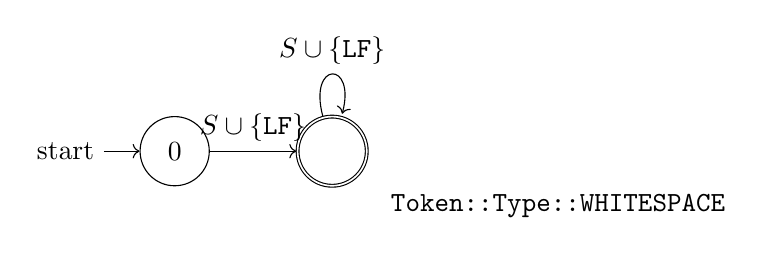
\begin{tikzpicture}
\node[state,initial] (q1) {$0$};
\coordinate[right of=q1] (tq1) {};
\node[state, right of=tq1, accepting] (q2) {};
\node [below right = 0.1cm and 0.3cm of q2]
    {\texttt{Token::Type::WHITESPACE}};
\draw
    (q1) edge[above, ->] node{$S\cup\{\texttt{LF}\}$} (q2)
    (q2) edge[loop above, ->] node{$S\cup\{\texttt{LF}\}$} (q2);
\end{tikzpicture}
\caption{States \& transitions for recognising
whitespace}
\end{figure}

\begin{figure}[H]
\centering
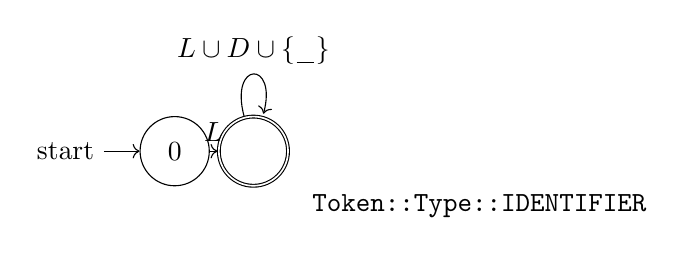
\begin{tikzpicture}
\node[state,initial] (q1) {$0$};
\node[state, right of=q1, accepting] (q2) {};
\node [below right = 0.1cm and 0.3cm of q2]
    {\texttt{Token::Type::IDENTIFIER}};
\draw
    (q1) edge[above, ->] node{$L$} (q2)
    (q2) edge[loop above, ->] node{$L \cup D \cup \{\texttt{\_}\}$} (q2);
\end{tikzpicture}
\caption{States \& transitions for recognising
identifiers/keywords}
\end{figure}

\begin{figure}[H]
\centering
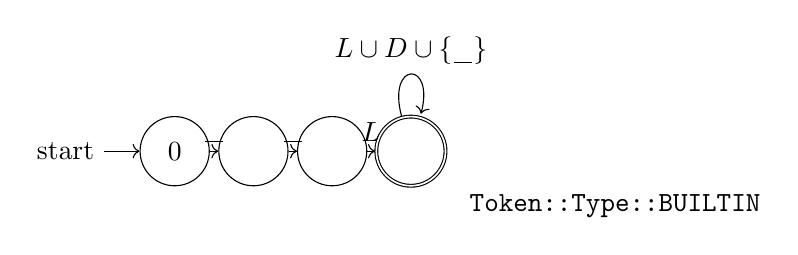
\begin{tikzpicture}
\node[state,initial] (q1) {$0$};
\node[state, right of=q1] (q2) {};
\node[state, right of=q2] (q3) {};
\node[state, right of=q3, accepting] (q4) {};
\node [below right = 0.1cm and 0.3cm of q4]
    {\texttt{Token::Type::BUILTIN}};

\draw
    (q1) edge[above, ->] node{\texttt{\_}} (q2)
    (q2) edge[above, ->] node{\texttt{\_}} (q3)
    (q3) edge[above, ->] node{$L$} (q4)
    (q4) edge[loop above, ->] node{$L \cup D \cup \{\texttt{\_}\}$} (q4);
\end{tikzpicture}
\caption{States \& transitions for recognising
builtins}
\end{figure}


\begin{figure}[H]
\centering
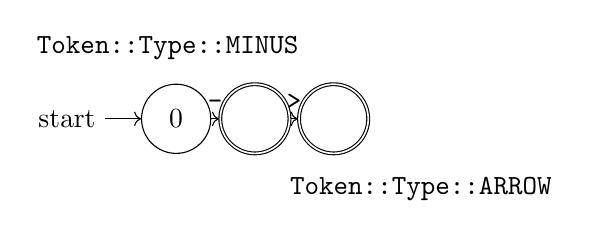
\begin{tikzpicture}
\node[state,initial] (q1) {$0$};
\node[state, right of=q1, accepting] (q2) {};
\node[state, right of=q2, accepting] (q3) {};
\node [above left = 0.3cm and -1cm of q2]
    {\texttt{Token::Type::MINUS}};
\node [below right = 0.3cm and -1cm of q3]
    {\texttt{Token::Type::ARROW}};
\draw
    (q1) edge[above, ->] node{\texttt{-}} (q2)
    (q2) edge[above, ->] node{\texttt{>}} (q3);
\end{tikzpicture}
\caption{States \& transitions for recognising
minus and arrow (\texttt{->})}
\end{figure}

\begin{figure}[H]
\centering
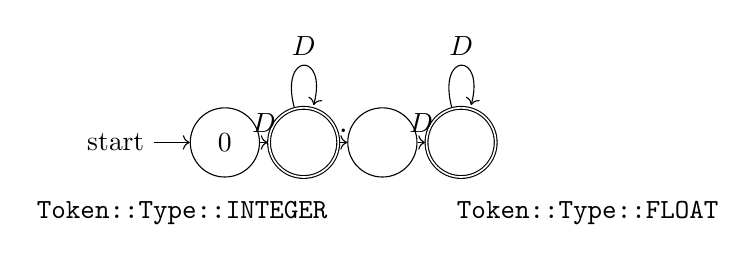
\begin{tikzpicture}
\node[state,initial] (q1) {$0$};
\node[state, right of=q1, accepting] (q2) {};
\node[state, right of=q2] (q3) {};
\node[state, right of=q3, accepting] (q4) {};
\node [below left = 0.3cm and -0.75cm of q2]
    {\texttt{Token::Type::INTEGER}};
\node [below right = 0.3cm and -0.5cm of q4]
    {\texttt{Token::Type::FLOAT}};
\draw
    (q1) edge[above, ->] node{$D$} (q2)
    (q2) edge[loop above, ->] node{$D$} (q2)
    (q2) edge[above, ->] node{\texttt{.}} (q3)
    (q3) edge[above, ->] node{$D$} (q4)
    (q4) edge[loop above, ->] node{$D$} (q4)
    ;
\end{tikzpicture}
\caption{States \& transitions for recognising
integers and floats}
\end{figure}

\begin{figure}[H]
\centering
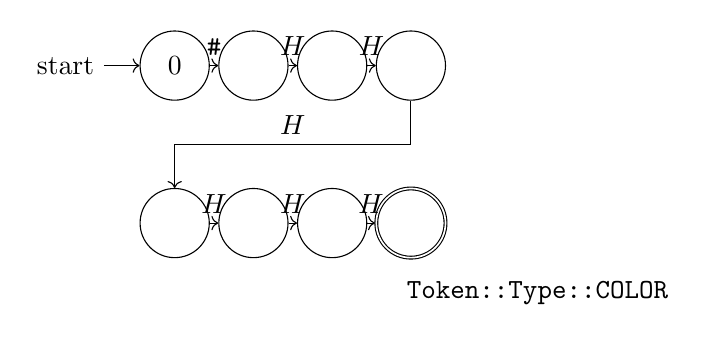
\begin{tikzpicture}
\node[state,initial] (q1) {$0$};
\node[state, right of=q1] (q2) {};
\node[state, right of=q2] (q3) {};
\node[state, right of=q3] (q4) {};

\coordinate[below of=q1] (bq1) {};
\coordinate[below of=q4] (bq4) {};

\node[state, below of=bq1] (q5) {};
\node[state, right of=q5] (q6) {};
\node[state, right of=q6] (q7) {};
\node[state, right of=q7, accepting] (q8) {};
\node [below right = 0.3cm and -0.5cm of q8]
    {\texttt{Token::Type::COLOR}};
\draw
    (q1) edge[above, ->] node{\texttt{\#}} (q2)
    (q2) edge[above, ->] node{$H$} (q3)
    (q3) edge[above, ->] node{$H$} (q4)
    (q4) -- (bq4)
    (bq4) edge[above] node{$H$} (bq1)
    (bq1) edge[->] (q5)
    (q5) edge[above, ->] node{$H$} (q6)
    (q6) edge[above, ->] node{$H$} (q7)
    (q7) edge[above, ->] node{$H$} (q8)
    ;
\end{tikzpicture}
\caption{States \& transitions for recognising
colours}
\end{figure}

\begin{figure}[H]
\centering
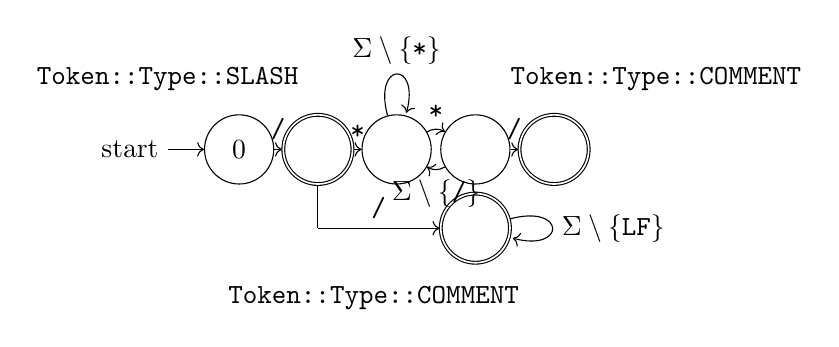
\begin{tikzpicture}
\node[state,initial] (q1) {$0$};
\node[state, right of=q1,accepting] (q2) {};

\coordinate[below of=q2] (bq2) {};

\node[state, right of=q2] (q4) {};
\node[state, right of=q4] (q5) {};
\node[state, right of=q5,accepting] (q6) {};

\node[state, below of=q5, accepting] (q3) {};

\node [above left = 0.3cm and -0.2cm of q2]
    {\texttt{Token::Type::SLASH}};

\node [above right = 0.3cm and -1cm of q6]
    {\texttt{Token::Type::COMMENT}};

\node [below left = 0.3cm and -1cm of q3]
    {\texttt{Token::Type::COMMENT}};

\draw
    (q1) edge[above, ->] node{\texttt{/}} (q2)
    (q2) -- (bq2)
    (bq2) edge[above, ->] node{\texttt{/}} (q3)
    (q3) edge[loop right, ->] node{$\Sigma \setminus \{\texttt{LF}\}$} (q3)
    (q2) edge[above, ->] node{\texttt{*}} (q4)
    (q4) edge[loop above, ->] node{$\Sigma \setminus \{\texttt{*}\}$} (q4)
    (q4) edge[above, bend left, ->] node{\texttt{*}} (q5)
    (q5) edge[below, bend left, ->] node{$\Sigma \setminus \{\texttt{/}\}$} (q4)
    (q5) edge[above, ->] node{\texttt{/}} (q6)
    ;
\end{tikzpicture}
\caption{States \& transitions for recognising
slashes and comments}
\end{figure}

\begin{figure}[H]
\centering
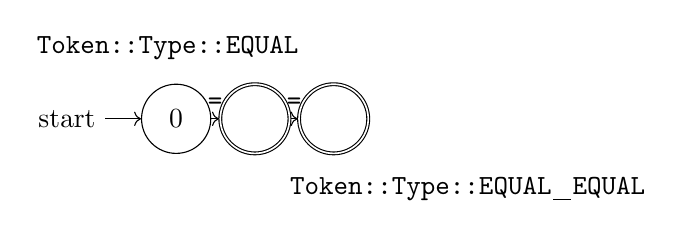
\begin{tikzpicture}
\node[state,initial] (q1) {$0$};
\node[state, right of=q1, accepting] (q2) {};
\node[state, right of=q2, accepting] (q3) {};
\node [above left = 0.3cm and -1cm of q2]
    {\texttt{Token::Type::EQUAL}};
\node [below right = 0.3cm and -1cm of q3]
    {\texttt{Token::Type::EQUAL\_EQUAL}};
\draw
    (q1) edge[above, ->] node{\texttt{=}} (q2)
    (q2) edge[above, ->] node{\texttt{=}} (q3);
\end{tikzpicture}
\caption{States \& transitions for assign
and is equal to}
\end{figure}

\begin{figure}[H]
\centering
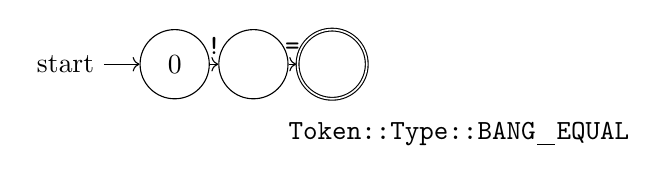
\begin{tikzpicture}
\node[state,initial] (q1) {$0$};
\node[state, right of=q1] (q2) {};
\node[state, right of=q2, accepting] (q3) {};
\node [below right = 0.3cm and -1cm of q3]
    {\texttt{Token::Type::BANG\_EQUAL}};
\draw
    (q1) edge[above, ->] node{\texttt{!}} (q2)
    (q2) edge[above, ->] node{\texttt{=}} (q3);
\end{tikzpicture}
\caption{States \& transitions for not equal to}
\end{figure}


\begin{figure}[H]
\centering
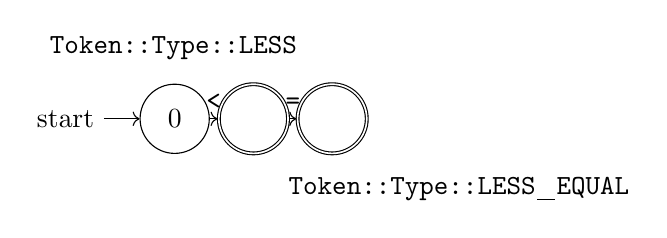
\begin{tikzpicture}
\node[state,initial] (q1) {$0$};
\node[state, right of=q1, accepting] (q2) {};
\node[state, right of=q2, accepting] (q3) {};
\node [above left = 0.3cm and -1cm of q2]
    {\texttt{Token::Type::LESS}};
\node [below right = 0.3cm and -1cm of q3]
    {\texttt{Token::Type::LESS\_EQUAL}};
\draw
    (q1) edge[above, ->] node{\texttt{<}} (q2)
    (q2) edge[above, ->] node{\texttt{=}} (q3);
\end{tikzpicture}
\caption{States \& transitions for less than
and less than or equal to}
\end{figure}

\begin{figure}[H]
\centering
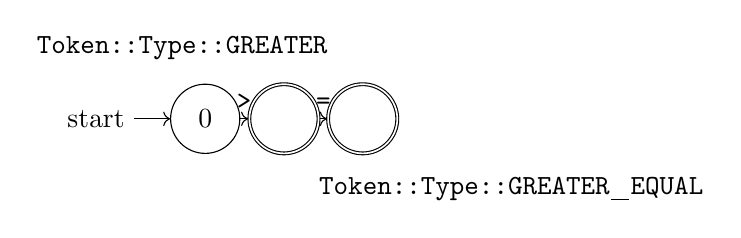
\begin{tikzpicture}
\node[state,initial] (q1) {$0$};
\node[state, right of=q1, accepting] (q2) {};
\node[state, right of=q2, accepting] (q3) {};
\node [above left = 0.3cm and -1cm of q2]
    {\texttt{Token::Type::GREATER}};
\node [below right = 0.3cm and -1cm of q3]
    {\texttt{Token::Type::GREATER\_EQUAL}};
\draw
    (q1) edge[above, ->] node{\texttt{>}} (q2)
    (q2) edge[above, ->] node{\texttt{=}} (q3);
\end{tikzpicture}
\caption{States \& transitions for greater than
and greater than or equal to}
\end{figure}


\begin{figure}[H]
\centering
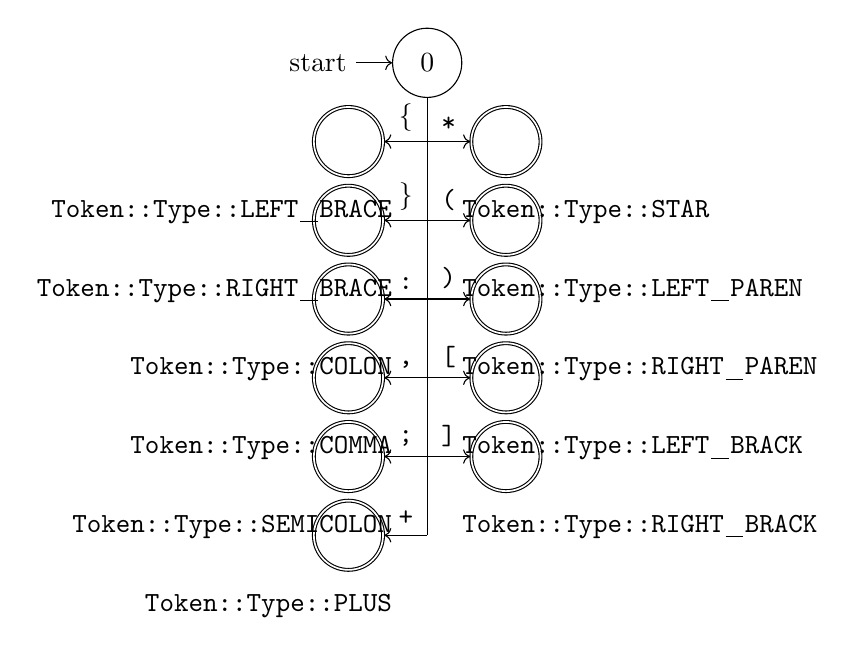
\begin{tikzpicture}
\node[state,initial] (q1) {$0$};

\coordinate[below of=q1] (b1) {};
\coordinate[below of=b1] (b2) {};
\coordinate[below of=b2] (b3) {};
\coordinate[below of=b3] (b4) {};
\coordinate[below of=b4] (b5) {};
\coordinate[below of=b5] (b6) {};

\node[state, right of=b1, accepting] (q2) {};
\node[state, below of=q2, accepting] (q3) {};
\node[state, below of=q3, accepting] (q4) {};
\node[state, below of=q4, accepting] (q5) {};
\node[state, below of=q5, accepting] (q6) {};

\node[state, left of=b1, accepting] (q7) {};
\node[state, below of=q7, accepting] (q8) {};
\node[state, below of=q8, accepting] (q9) {};
\node[state, below of=q9, accepting] (q10) {};
\node[state, below of=q10, accepting] (q11) {};
\node[state, below of=q11, accepting] (q12) {};

\node [below right = 0.3cm and -1cm of q2]
    {\texttt{Token::Type::STAR}};
\node [below right = 0.3cm and -1cm of q3]
    {\texttt{Token::Type::LEFT\_PAREN}};
\node [below right = 0.3cm and -1cm of q4]
    {\texttt{Token::Type::RIGHT\_PAREN}};
\node [below right = 0.3cm and -1cm of q5]
    {\texttt{Token::Type::LEFT\_BRACK}};
\node [below right = 0.3cm and -1cm of q6]
    {\texttt{Token::Type::RIGHT\_BRACK}};

\node [below left = 0.3cm and -1cm of q7]
    {\texttt{Token::Type::LEFT\_BRACE}};
\node [below left = 0.3cm and -1cm of q8]
    {\texttt{Token::Type::RIGHT\_BRACE}};
\node [below left = 0.3cm and -1cm of q9]
    {\texttt{Token::Type::COLON}};
\node [below left = 0.3cm and -1cm of q10]
    {\texttt{Token::Type::COMMA}};
\node [below left = 0.3cm and -1cm of q11]
    {\texttt{Token::Type::SEMICOLON}};
\node [below left = 0.3cm and -1cm of q12]
    {\texttt{Token::Type::PLUS}};

\draw
    (q1) -- (b1)
    (b1) -- (b2)
    (b2) -- (b3)
    (b3) -- (b4)
    (b4) -- (b5)
    (b5) -- (b6)
    ;

\draw
    (b1)  edge[above, ->] node{\texttt{*}} (q2)
    (b2) edge[above, ->] node{\texttt{(}} (q3)
    (b3) edge[above, ->] node{\texttt{)}} (q4)
    (b4) edge[above, ->] node{\texttt{[}} (q5)
    (b5) edge[above, ->] node{\texttt{]}} (q6)

    (b1) edge[above, ->] node{\texttt{\{}} (q7)
    (b2) edge[above, ->] node{\texttt{\}}} (q8)
    (b3) edge[above, ->] node{\texttt{:}} (q9)
    (b4) edge[above, ->] node{\texttt{,}} (q10)
    (b5) edge[above, ->] node{\texttt{;}} (q11)
    (b6) edge[above, ->] node{\texttt{+}} (q12)
    ;
\end{tikzpicture}
\caption{States \& transitions for single letter tokens}
\end{figure}

\subsubsection{The Builder \& Director}

Each sequence of states present is directly
represented in code within the
\texttt{LexerDirector} using methods provided by
the \texttt{LexerBuilder}.

\lstinputlisting[
firstline=297,
lastline=309,
caption={Code specification of
the comments in the \texttt{LexerDirector}
(lexer/LexerDirector.cpp)},
label=lst:commenttransitions
]{lexer/LexerDirector.cpp}

The \texttt{LexerBuilder} keeps track of these
transitions using less efficient data structures
such as hash maps (\texttt{std::unordered\_map})
and sets (\texttt{std::unordered\_set}).

Then the \texttt{build()} method processes the
user defined transitions and normalises everything
into a single transition table for use in a DFSA.
Additionally, it also produces two other
artefacts. The first is called
\texttt{categoryIndexToChecker}. It is a hash map
from the index of a category to a lambda function
which takes a character as input and returns true
or false.

The lambdas and the category indices are also
registered by the user. See \listref{checkerreg}
for a registration example. Additionally, the
category indices although they are integers for
readability they are defined as an enumeration.

\lstinputlisting[
firstline=51,
lastline=58,
caption={Registration of the hexadecimal category
checker (lexer/LexerDirector.cpp)},
label=lst:checkerreg
]{lexer/LexerDirector.cpp}

The second artefact produced by the builder is
also a hash map from final states to their
associated token type.

The transition table is then passed onto the DFSA.
And the DFSA, and the two artefacts are passed
onto the Lexer class.

\lstinputlisting[
firstline=210,
lastline=224,
caption={Constructions of the Lexer
(lexer/LexerBuilder.cpp)},
]{lexer/LexerBuilder.cpp}

\subsubsection{The Actual Lexer}

The lexer's core is as was described during the
lectures and the core/main method is
\texttt{simulateDFSA()}.

It also has a number of very important auxiliary
methods and behavioural changes. Specifically, the
\texttt{updateLocationState()}, see
\listref{updateloc}, is critical for providing
adequate error messages both during the current
stage and for later stages. This function is
called every time a lexeme is consumed allowing
the lexer to keep track of where in the file it
is, in terms of lines and columns.

\lstinputlisting[
firstline=110,
lastline=122,
caption={The \texttt{updateLocationState()} lexer
method (lexer/Lexer.cpp)},
label=lst:updateloc
]{lexer/Lexer.cpp}

Additionally, if an invalid / non-accepting state
is reached the invalid lexeme is consumed and the
user is warned, see \listref{lexererrors}. After
this the lexer, is left in a still operational state.
Hence, \texttt{nextToken()} can be used again.

 This is critical to provide users of the
 \texttt{PArL} compiler with a list of as many
 errors as possible, since it would be a bad
 experience to have to constantly run the
 \texttt{PArL} compiler to see the next error.

\lstinputlisting[
firstline=56,
lastline=84,
caption={Error handling mechanism in the
\texttt{nextToken()} lexer method
(lexer/Lexer.cpp)},
label=lst:lexererrors
]{lexer/Lexer.cpp}

\subsubsection{Hooking up the Lexer to the Runner}

The \texttt{Runner} class is the basic structure
which connects all the stages of the
compiler together together.

In this case the Runner passes in a reference to
the lexer into the parser, this allows the parser
to request tokens and they are computed on demand
improving overall performance. Additionally, this
has the benefit of allowing the parsing of larger
and multiple files since, the parser is no longer
limited by the amount of usable memory, since it
does not need to load the whole file.

However, in this case no such optimisation is
present.

\lstinputlisting[
firstline=22,
lastline=28,
caption={The Runner constructor passes
\texttt{mLexer} into the Parser constructor
(runner/Runner.cpp)}
]{runner/Runner.cpp}

\section{The AST \& Parsing}

\subsection{Modified EBNF}

\setlength{\grammarparsep}{8pt plus 1pt minus 1pt} % increase separation between rules
\setlength{\grammarindent}{10em} % increase separation between LHS/RHS

Some modifications were applied to the original EBNF. Some of
the modifications were either motivated by improved user
experience, a more uniform mechanism and others to reduce
complexity further down the pipeline.

\begin{center}
\begin{grammar}
<Letter> ::= `A'-`Z' | `a'-`z'

<Digit> ::= `0'-`9'

<Hex> ::= `A'-`F' | `a'-`F' | <Digit>

<Identifier> ::= <Letter> \{`\_' | <Letter> | <Digit>\}

<BooleanLiteral> ::= `true' | `false'

<IntegerLiteral> ::= <Digit> \{<Digit>\}

<FloatLiteral> ::= <Digit> \{<Digit>\} `.' <Digit> \{<Digit>\}

<ColorLiteral> ::= `\#' <Hex> <Hex> <Hex> <Hex> <Hex> <Hex>

<ArrayLiteral> ::= `[' [<Epxr> \{`,' <Epxr>\}] `]'

<PadWidth> ::= `\_\_width'

<PadHeight> ::= `\_\_height'

<PadRead> ::= `\_\_read' <Epxr> `,' <Epxr>

<PadRandomInt> ::= `\_\_random\_int' <Epxr>

<Literal> ::= <BooleanLiteral>
\alt <IntegerLiteral>
\alt <FloatLiteral>
\alt <ColorLiteral>
\alt <ArrayLiteral>
\alt <PadWidth>
\alt <PadHeight>
\alt <PadRead>
\alt <PadRandomInt>

<Type> ::= (`bool' | `int' | `float' | `color') [ `[' <IntegerLiteral> `]' ]

<SubEpxr> ::= `(' <Epxr> `)'

<Variable> ::= <Identifier>

<ArrayAccess> ::= <Identifier> `[' <Epxr> `]'

<FunctionCall> ::= <Identifier> `(' [<Epxr> \{`,' <Epxr>\}] `)'

<Epxr> ::= <LogicOr> [`as' <Type>]

<LogicOr> ::= <LogicAnd> \{`or' <LogicAnd>\}

<LogicAnd> ::= <Equality> \{`and' <Equality>\}

<Equality> ::= <Comparison> \{(`==' | `!=') <Comparison>\}

<Comparison> ::= <Term> \{(`<' | `<=' | `>' | `>=') <Term>\}

<Term> ::= <Factor> \{(`+' | `-') <Factor>\}

<Factor> ::= <Unary> \{(`*' | `/') <Unary>\}

<Unary> ::= (`-' | `not') <Unary> | <Primary>

<Primary> ::= <Literal>
\alt <SubExpr>
\alt <Variable>
\alt <ArrayAccess>
\alt <FunctionCall>

<Program> ::= \{<Stmt>\}

<Stmt> ::= <Block>
\alt <VaribaleDecl> `;'
\alt <FunctionDecl>
\alt <Assignment> `;'
\alt <PrintStmt> `;'
\alt <DelayStmt> `;'
\alt <WriteBoxStmt> `;'
\alt <WriteStmt> `;'
\alt <ClearStmt> `;'
\alt <IfStmt>
\alt <ForStmt>
\alt <WhileStmt>
\alt <ReturnStmt> `;'

<Block> ::= `\{' \{<Stmt>\} `\}'

<VariableDecl> ::= `let' <Identifier> `:' <Type> `='
<Epxr>

<FormalParam> ::= <Identifier> `:' <Type>

<FunctionDecl> ::= `fun' <Identifier> `(' [ <ForamlParam>
\{`,' <FormalParam>\}] `)' `->' <Type> <Block>

<Assignment> ::= <Identifier> [`[' <Epxr> `]'] `='
<Epxr>

<PrintStmt> ::= `\_\_print' <Epxr>

<DelayStmt> ::= `\_\_delay' <Epxr>

<WriteBoxStmt> ::= `\_\_write\_box' <Epxr>`,'
<Epxr>`,'<Epxr>`,' <Epxr>`,'<Epxr>

<WriteStmt> ::= `\_\_write' <Epxr>`,' <Epxr>`,'<Epxr>

<ClearStmt> ::= `\_\_clear' <Epxr>

<IfStmt> ::= `if' `(' <Expr> `)' <Block> [`else' <Block>]

<ForStmt> ::= `for' `(' [<VariableDecl>] `;' <Expr> `;'
[<Assignment>] `)' <Block>

<WhileStmt> ::= `while' `(' <Expr> `)' <Block>

<ReturnStmt> ::= `return' <Expr>
\end{grammar}
\end{center}

\subsubsection{Improved Precedence}

So, the minor changes which improve programmer usability are the
additions of a number of other expression stages, such as
$\langle$LogicOr$\rangle$, $\langle$LogicAnd$\rangle$, etc. The
main reason for the addition of such rules is to further enforce
a more natural operation precedence. For example a programmer
often expects that comparison operators such as \texttt{<} and
\texttt{>} bind tighter than \texttt{and} or \texttt{or}, hence
the compiler needs to make sure that comparison operators are
executed before logical operators, and this can be enforced by
the grammar itself hence the changes.

\subsubsection{A Better Type System}




\section{Semantic Analysis}

\subsection{Phases \& Design}

As described in \ref{eyecandy} the Semantic Analysis phase
should be split into a number of sub-phases specifically: symbol
resolution, de-sugaring/type inference and type checking.

However, these steps can be combined together into a single step
phase. There a benefits and downsides to both approaches. The
main benefit of using the first approach is a reduction in
algorithmic complexity. The logic can be separated into
different phases with ease and information from one phase can be
propagated to another. The downside of this approach is that it
actually adds more code for maintenance, since each individual
sub-phase will probably need to be implemented as its own
visitor. The other down side is error management. If an error
occurs in a particular phase since said phase is completely
disjoint from the phases after it a mechanism for propagation
needs to be devised which again further increases complexity. Of
course by the very nature of this argument the monolithic
approach does not suffer for the issues that the sub-phases
approach has. However, it significantly increases complexity
since all sub-phases are being done in a single phase. The other
more glaring issue is the fact that it is much more difficult to
resolve symbols before-hand.

You would want to do so to allow for the location of function
declarations in code to not effect resolution, that is, a
function can be called before it is referenced.

Unfortunately, due to the fact that compiler development was an
organic process and not too much time was spend on deliberation
the semantic analysis phase became monolithic, and hence it
suffers from the issues described above. Of course, this means
location agnostic function declaration are currently \emph{not}
supported by the compiler.

\subsection{The Environment Tree}

Some terminology is required to properly describe the number of
structures which will be used in this section. The following
terms are critical and need to be differentiated properly:

\begin{itemize}
    \item \texttt{SymbolTable}
    \item \texttt{SymbolTableStack}
    \item \texttt{Environment}
    \item \texttt{EnvStack}
    \item \texttt{RefStack}
\end{itemize}

During semantic analysis there is a need for specific data
structures which facilitate scoping rules, type checking, etc.

The most basic data structure which achieves this, is a single
\texttt{SymbolTable}. A symbol table in its simplest form is a
wrapper around a hash map, whose keys are identifiers and values
are \texttt{Symbol}s or any structure which is capable of
storing variable and function signatures.

This approach is quite limiting since it restricts developers
and user of the language to a single global scope. Therefore,
this is structure is not a sufficient solution for most
toy-languages let alone production ready languages.

A better solution is using a stack of symbol tables. This allows
symbol tables to shadow each other allowing for the reuse of
identifiers. Additionally, this further opens up the possibility
of implementing modules at the language-level. The likelihood
that names will be reused across different modules is quite high
and being able to scope modules so they do not interfere with
global scope and each other is necessary for any sufficiently
large project.

\begin{figure}[H]
\centering
\begin{mdframed}[backgroundcolor=UMPaleRed]
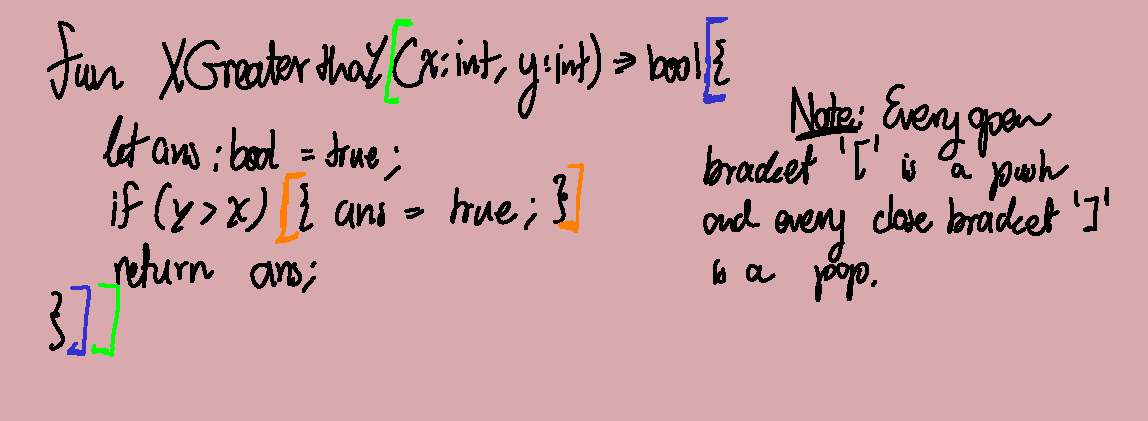
\includegraphics[width=\linewidth]{scopedcode.pdf}
\end{mdframed}
\caption{A \texttt{PArL} function with annotated scopes}
\label{fig:scopeannotatedcode}
\end{figure}

The basic premise of using a symbol table stack is described in
\algref{basicsymboltablestack} and \figref{graphicaldecpiction}.
A new symbol table, also referred to as a scope, is pushed onto
a stack only for specific types of AST nodes. The node is then
processed, were ``processing'' often times means considering all
the sub-children of the node, and when processing terminates the
scope is popped. In the context of a purely stack based
implementation this implies that, scopes are only temporary that
is they are lost after being popped.

\begin{algorithm}[H]
\KwData{$N$ the AST node, $S$ the symbol table stack}

\Begin{
    \If{$N$ opens a scope}{
        PushScope($S$)\;
    }
    ProcessNode($N$)\;
    \If{$N$ opens a scope}{
        PopScope($S$)\;
    }
}

\caption{Basic description of \texttt{SymbolTableStack} usage}
\label{alg:basicsymboltablestack}
\end{algorithm}

\begin{figure}[H]
\centering
\begin{mdframed}[backgroundcolor=UMPaleRed]
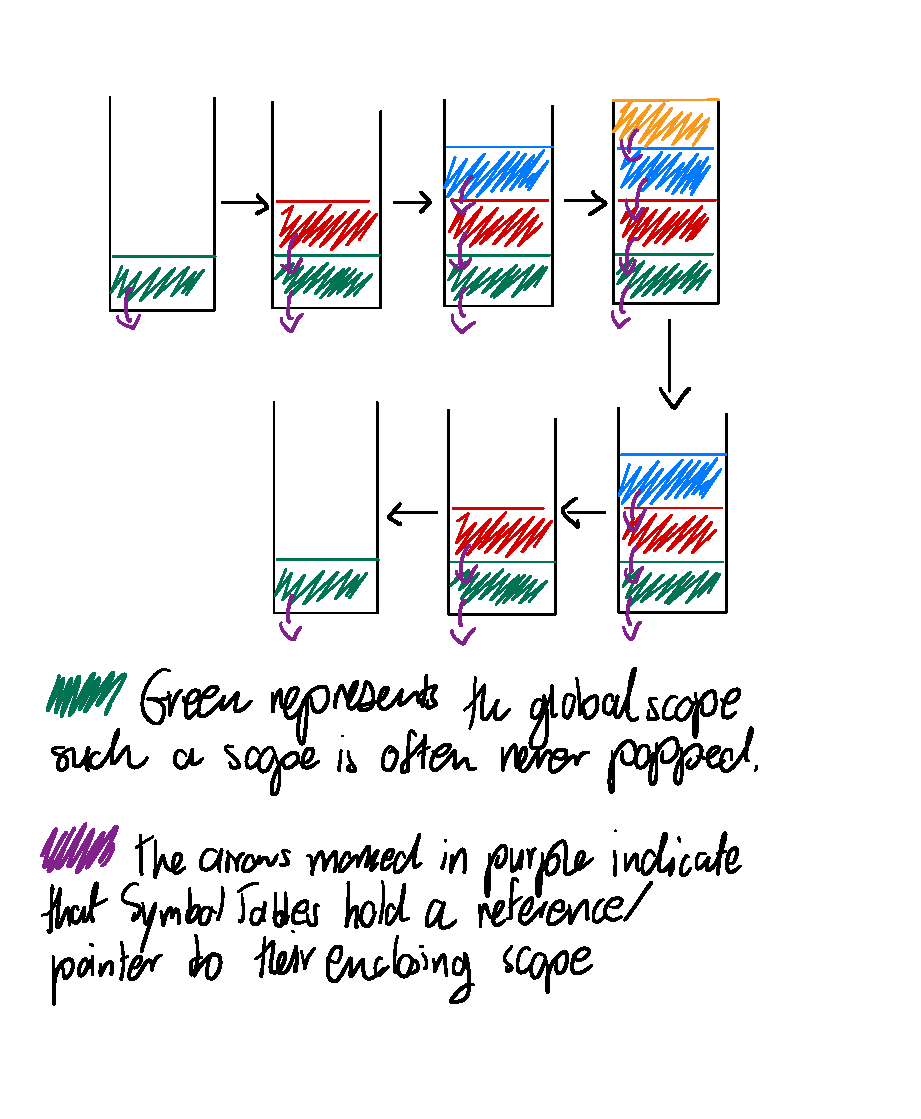
\includegraphics[width=\linewidth]{symboltablestack.pdf}
\end{mdframed}
\caption{Behaviour of the \texttt{SymbolTableStack} when
considering the code in \figref{scopeannotatedcode}}
\label{fig:graphicaldecpiction}
\end{figure}

The main advantage of using this approach is that the
worst case memory usage is $O(DI)$ where $D$ is the length of a
longest chain of open scopes and $I$ is the size of largest
number of variable declarations within a scope.

However, due to the temporary nature of this approach it does
not lend itself well to a multi-phase approach. This is because
at each phase \texttt{SymbolTable}s have to be regenerated
increase the complexity of each individual phase.

Instead a different approach shall be used. This approach uses
an
\href{https://craftinginterpreters.com/statements-and-state.html#nesting-and-shadowing}{Environment
Tree} and it has also been inspired by
\href{https://craftinginterpreters.com/}{Crafting Interpreters}.

The notion of an \texttt{Environment} is essentially, the same
as a \texttt{SymbolTable}. The only significant change is the
addition of vector of unique pointers to other environments, see
\listref{envclass}.

\begin{lstlisting}[escapechar=!,caption={The
\texttt{Environment} class with \texttt{mChildren} highlighted
(backend/Environment.hpp)}, label=lst:envclass]
class Environment {
   public:
    enum class Type {
        GLOBAL,
        IF,
        ELSE,
        FOR,
        WHILE,
        FUNCTION,
        BLOCK
    };

    void addSymbol(
        std::string const& identifier,
        Symbol const& Symbol
    );
    [[nodiscard]] std::optional<Symbol> findSymbol(
        std::string const& identifier
    ) const;
    Symbol& getSymbolAsRef(std::string const& identifier);

    [[nodiscard]] Environment* getEnclosing() const;
    void setEnclosing(Environment* enclosing);

    [[nodiscard]] Type getType() const;
    void setType(Type type);

    [[nodiscard]] std::optional<std::string> getName(
    ) const;
    void setName(const std::string& name);

    std::vector<std::unique_ptr<Environment>>& children();

    [[nodiscard]] bool isGlobal() const;

    [[nodiscard]] size_t getIdx() const;
    void incIdx();
    void incIdx(size_t inc);

    [[nodiscard]] size_t getSize() const;
    void setSize(size_t size);

   private:
    std::unordered_map<std::string, Symbol> mMap{};
    Type mType{Type::GLOBAL};
    std::optional<std::string> mName{};
    Environment* mEnclosing{nullptr};
    !\colorbox{UMPaleRed}{std::vector<std::unique_ptr<Environment>> mChildren\{\};}!
    size_t mSize{0};
    size_t mIdx{0};
};
\end{lstlisting}

The additional fields present in the \texttt{Environment} class
are there to cater for the needs of each of the phases.

Specifically, \texttt{mType} and \texttt{mName} are used during
semantic analysis and \texttt{mSize} and \texttt{mIdx} are used
during code generation.

Additionally, it is preferable if the interface with which the
phases interact with the \texttt{Environment} tree is identical
to that of a \texttt{SymbolTableStack}, that is the same
\texttt{push()} and \texttt{pop()} methods are used.

Now to facilitate this another two classes need to be defined
\texttt{EnvStack} and \texttt{RefStack}. The main difference
between \texttt{EnvStack} and \texttt{RefStack} is that the
purpose of \texttt{EnvStack} is to construct the
\texttt{Environment} tree whilst \texttt{RefStack} traverses the
environment tree. Due to this \texttt{RefStack} is only required
during the symbol resolution. However, in current implementation
since symbol resolution is combined with type checking, the
Environment tree is generated at the same time as it is being
type checked.

Additionally, in both an \texttt{EnvStack} and a
\texttt{RefStack}, the creation and traversal of the Environment
tree are managed via the \texttt{push()} and \texttt{pop()}
methods.

In an \texttt{EnvStack} \texttt{push()} works by creating a new
environment, setting the enclosing environment to the current
environment and changing the current environment to to the new
environment, see \listref{evnstackpush}. \texttt{pop()} makes
use of the \texttt{mEnclosing} field in the current environment
and just sets the current environment to the enclosing
environment essentially moving up an environment, see
\listref{popenvstack}.

\lstinputlisting[linerange={12-22}, caption={The
\texttt{pushEnv()} method in the \texttt{EnvStack} class
(analysis/EnvStack.cpp)}, label=lst:envstackpush
]{analysis/EnvStack.cpp}

\lstinputlisting[linerange={24-28}, caption={The
\texttt{popEnv()} method in the \texttt{EnvStack} class
(analysis/EnvStack.cpp)}, label=lst:envstackpop
]{analysis/EnvStack.cpp}

The implementations in \texttt{RefStack} are however a bit more
involved. This is because the program has to be able to perform
a step-wise left-first depth-first traversal. The best way
to do this is to make use of a stack and the algorithms
in \listref{refpush} and \listref{refpop}.

\lstinputlisting[linerange={7-17}, caption={The
\texttt{pushEnv()} method in the \texttt{RefStack} class
(ir\_gen/RefStack.cpp)}, label=lst:refpush
]{ir\_gen/RefStack.cpp}

\lstinputlisting[linerange={37-43}, caption={The
\texttt{popEnv()} method in the \texttt{RefStack} class
(ir\_gen/RefStack.cpp)}, label=lst:refpop
]{ir\_gen/RefStack.cpp}

See \figref{refstackdryrun}, for the initial segments of a
traversal. The important thing to note here is that the
correctness of the traversal entirely depends on the usage of
\texttt{push()} and \texttt{pop()}. If used incorrectly the
traversal might be incorrect or the program might crash. Of
course, this is only an implementation detail that is if used
correctly by the compiler developer no such issue should occur.

\begin{figure}[H]
\centering
\begin{mdframed}[backgroundcolor=UMPaleRed]
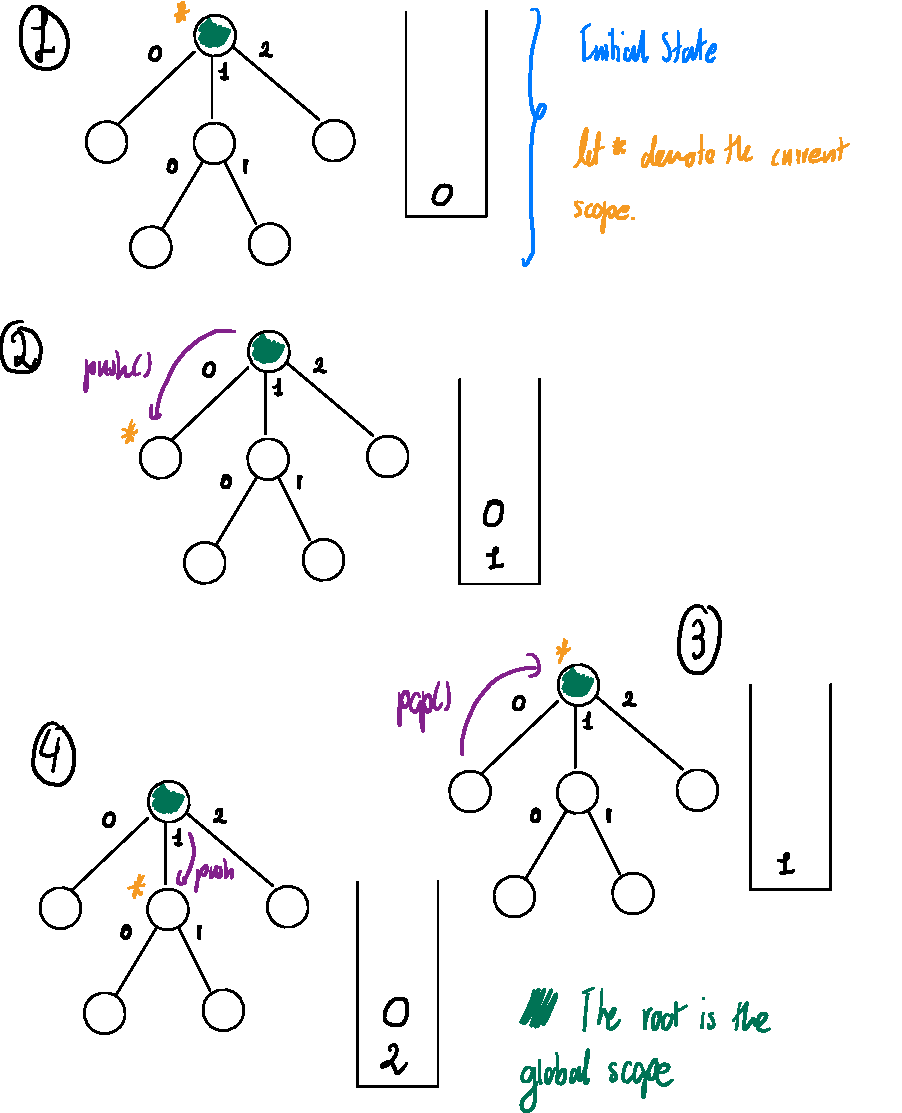
\includegraphics[width=\linewidth]{refstackdryrun.pdf}
\end{mdframed}
\caption{The initial steps of a traversal performed by
\texttt{RefStack}}
\label{fig:refstackdryrun}
\end{figure}

\subsection{Semantic Analysis}

Having the necessary data structures in place the discussion
will now revolve around Semantic Analysis i.e. the process of
making sure the meaning of the program is correct.

There are four main areas of interest which shall be discussed:
the symbol type, symbol registration/search, type checking and a
unique subset of type checking, return value type verification.

\subsection{The \texttt{Symbol} Type}

Within \texttt{PArL}

This minor change removes the need to throw away Environments
and they can be passed on from one phase to another.

\begin{figure}[H]
\centering
\begin{mdframed}[backgroundcolor=UMPaleRed]
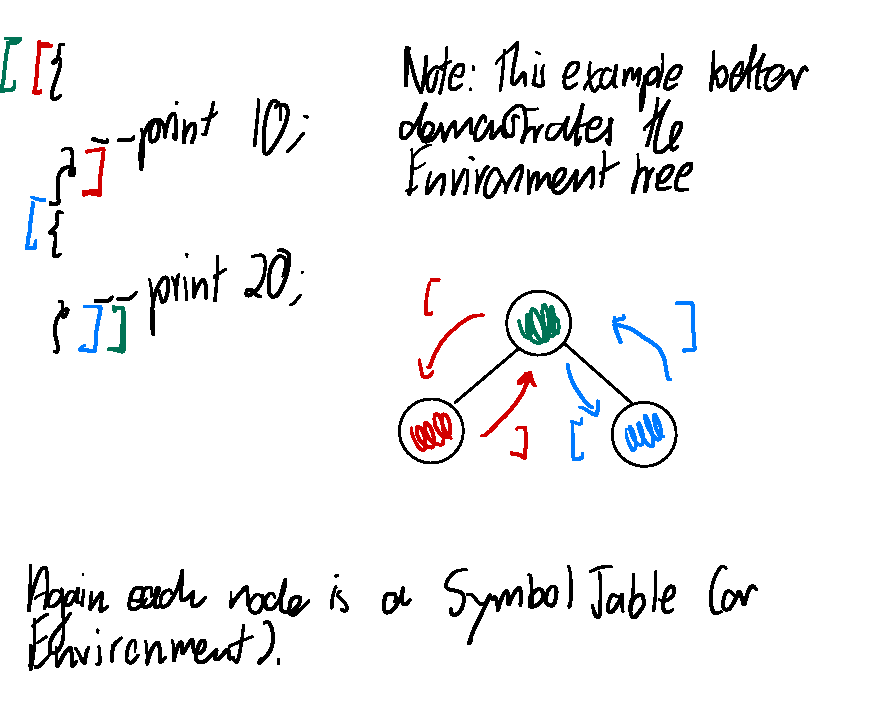
\includegraphics[width=\linewidth]{scopedcode2.pdf}
\end{mdframed}
\caption{Construction of an \texttt{Environment} tree}
\label{fig:scopedcode2}
\end{figure}

The Environment tree is a data structure

\begin{itemize}
    \item Describe Symbol Table.
    \item Describe each element of the symbol table.
    \item Describe the tree approach.
    \item attribute the tree approach to Robert Nystrom as well.
    \item describe the main advantage/disadvantage of using a environment
        approach.
    \item describe the main advantage/disadvantage of using a symbol stack
        approach.
\end{itemize}

\section{Code Generation}

Having completed semantic analysis, the compiler
can proceed to code generation.

\subsection{Passing on the \texttt{Environment} Tree}

Before, proceeding onto to the details of code generation it is
important to note that here is were all the upfront work that
was put into using \texttt{Environment} trees, pays off. This is
because there is no need to re-stablish the types of any of the
variables, at any scope.

\begin{lstlisting}[caption={Getting the global environment from
the \texttt{AnalysisVisitor} and passing it on for reordering
and code generation (runner/Runner.cpp).}]
std::unique_ptr<Environment> environment =
    mAnalyser.getEnvironment();

ReorderVisitor reorder{};

reorder.reorderAst(ast.get());

if (mParserDbg) {
    debugParsing(ast.get());
}

reorder.reorderEnvironment(environment.get());

GenVisitor gen{environment.get()};
\end{lstlisting}

\subsubsection{The \texttt{TypeVisitor} Class}

Having said that there is still the need to recompute the types
of expressions since the type of a composite expression e.g.
\texttt{2 + 3} cannot be stored in an \texttt{Environment}. To
handle this another visitor, this time called
\texttt{TypeVisitor} was created.

\begin{todo}
In the event that type checking/generation is completely
delegated to the \texttt{TypeVisitor}, future version of
compiler can drop usage of \texttt{Environment} trees in favour
of re-computing types as requested. Additionally, such a change
improves memory usage in exchange for time as described in
\ref{sss:memoryadvantage}.
\end{todo}

\begin{lstlisting}[caption={The \texttt{visit(FunctionCall *)}
method in the \texttt{TypeVisitor} class
(ir\_gen/TypeVisitor.cpp).}, label=lst:recomputefunctype]
void TypeVisitor::visit(core::FunctionCall *expr) {
    std::optional<Symbol> symbol{
        findSymbol(expr->identifier, mRefStack.getGlobal())
    };

    mReturn = symbol->as<FunctionSymbol>().returnType;

    expr->core::Expr::accept(this);
}
\end{lstlisting}

Currently, a \texttt{TypeVisitor} is given a \texttt{RefStack}
for \texttt{Environment} access and its main capability is
re-calculating the type of \textbf{already} type-checked
expressions (see \listref{recomputefunctype}).

\begin{marker}
Usage of a \texttt{TypeVisitor} on a non-type-checked expression
will at best crash and at worst still work, leading to undefined
behaviour.
\end{marker}

\subsection{Reordering}\label{sss:reordersec}

Due to the fact that the \texttt{PArDis} VM Simulator expects
all functions to be defined before the \texttt{.main} segment,
which in the case of \texttt{PArL} is everything not in a
function declaration, a solution needs to be devised to ensure
that this order requirement is satisfied.

A solution to this problem can be achieved by reordering the AST
and the \\ \texttt{Environment}s. Since function declarations can
only exist in global scope, moving them such that they are the
first statements, which are encountered, is a sufficient
modification to ensure code generation as required by the VM.

\begin{todo}
Currently the compiler has support for named scopes (see
backend/Environemnt.cpp, lines 25 and 34). With a specially
designed naming scheme to uniquely identify each scope, support
for nested functions can be enable by mangling function names
with scope names and lifting function declarations into global
scope.
\end{todo}

This approach required two visitors, named
\texttt{IsFunctionVisitor} and \\ \texttt{ReorderVisitor}, and a
function, \texttt{reorderEnvironment()} (the choice to embed it
into the \texttt{ReorderVisitor} was arbitrary).

The \texttt{IsFunctionVisitor} is quite self-explanatory, it is
a very simple visitor with an exposed method \texttt{check()},
which returns true only if a node is a function declaration.

\begin{lstlisting}[caption={The \texttt{reorder()} method in the
\texttt{ReorderVisitor} class (preprocess/ReorderVisitor.cpp).}]
void ReorderVisitor::reorder(
    std::vector<std::unique_ptr<core::Stmt>> &stmts
) {
    for (auto &stmt : stmts) {
        if (isFunction.check(stmt.get())) {
            mFuncQueue.push_back(std::move(stmt));
        } else {
            mStmtQueue.push_back(std::move(stmt));
        }
    }

    stmts.clear();

    for (auto &stmt : mFuncQueue) {
        stmts.push_back(std::move(stmt));
    }

    for (auto &stmt : mStmtQueue) {
        stmts.push_back(std::move(stmt));
    }

    reset();
}
\end{lstlisting}

The \texttt{ReorderVisitor} implements a method
\texttt{reorder()}, which is called only for program and block
nodes. The \texttt{reorder()} makes use of two queues. The first
queue keeps track of function declarations and the second queue
keeps track of everything else. The \texttt{reorder()} method
traverse the provided statement vector and enqueues statements
in there respective queues. Then the elements of the first queue
are dequeued back into the vector followed by  the elements of
second queue. Due to the usage of queues this essentially moves
all function declarations (in their original order) as the first
elements of the statements vector. The visitor is then accepted
by all the reordered statements.

\begin{note}
The visitor is accepted by the reordered statements, to cater
for the case when function declarations are also present in
other scopes not just the global scope. However, this is
currently not the case (see analysis/AnalysisVisitor.cpp, line
955).
\end{note}

\subsection{Function Declarations}

Due to the reordering described in \ref{sss:reordersec}, the
first nodes to be emitted are function declarations.

\begin{lstlisting}[escapechar=!, caption={The
\texttt{visit(FunctionDecl *)} method in the \texttt{GenVisitor}
class (ir\_gen/GenVisitor.cpp).}, label=lst:genfuncdecl]
void GenVisitor::visit(core::FunctionDecl *stmt) {
    Environment *nextEnv = mRefStack.peekNextEnv();

    size_t aritySize{0};

    for (auto &stmt : stmt->params) {
        aritySize +=
            !\colorbox{UMPaleRed}{mDeclCounter.count(stmt.get(),\
            nextEnv);}!
    }

    !\colorbox{UMPaleRed}{emit_line(".\{\}",\
    stmt->identifier);}!

    mRefStack.pushEnv(aritySize);

    for (auto &param : stmt->params) {
        !\colorbox{UMPaleRed}{param->accept(this);}!
    }

    stmt->block->accept(this);

    mRefStack.popEnv();
}
\end{lstlisting}

Again for code generation two more visitors apart from the
\texttt{TypeVisitor} were used. These are the
\texttt{GenVisitor} and the \texttt{VarDeclCountVisitor}.

\begin{lstlisting}[caption={The \texttt{visit(VariableDecl *)}
method in the \texttt{VarDeclCountVisitor} class
(ir\_gen/VarDeclCountVisitor.cpp)}, label=lst:vardeclcount]
void VarDeclCountVisitor::visit(core::VariableDecl *stmt) {
    std::optional<Symbol> symbol =
        mEnv->findSymbol(stmt->identifier);

    auto &variable = symbol->asRef<VariableSymbol>();

    mCount += variable.type.is<core::Array>()
                  ? variable.type.as<core::Array>().size
                  : 1;
}
\end{lstlisting}

The \texttt{GenVisitor} as its name suggest is the main visitor
which produces the VM instructions. The
\texttt{VarDeclCountVisitor} is an additional visitor which is
used to calculate the size of the memory required when opening a
frame on the VM.

\begin{note}\label{sss:framesizecalc}
Within the VM memory is implemented in the form a JavaScript
array. This means that there are no restrictions on how big a
single location is, for this reason there is no true standard
unit of size. However, it is implicitly assumed that the base
types: \texttt{bool}, \texttt{int}, \texttt{float} and
\texttt{color} all occupy single a unit. Hence, when calculating
the size of for example \texttt{int[4]} the
\texttt{VarDeclCountVisitor} returns $4$ (see
\listref{vardeclcount}).
\end{note}

\begin{lstlisting}[caption={The \texttt{emit\_line()} method in
the \texttt{GenVisitor} class (ir\_gen/GenVisitor.cpp).},
label=lst:emitline]
template <typename... T>
void emit_line(fmt::format_string<T...> fmt, T &&...args) {
    mCode.push_back(fmt::format(fmt, args...));
}
\end{lstlisting}

On the other hand, the main mechanism with which the
\texttt{GenVisitor} emits VM code is \texttt{emit\_line()}.
Again similar to \texttt{error()} and \texttt{warning()} (from
other visitors), \texttt{emit\_line()} wraps an fmtlib function
(see \listref{genfuncdecl} and \listref{emitline}).

In the context of function declarations the only significant
usage of \texttt{emit\_line()} is to output the identifier of
the function.

\subsection{Scopes, Variable (or Formal Parameter) Declarations
\& Variable Accesses}

\begin{lstlisting}[caption={The \texttt{visit(VariableDecl *)}
method in the \texttt{GenVisitor} class
(ir\_gen/GenVisitor.cpp).}, label=lst:formalparam]
void GenVisitor::visit(core::VariableDecl *stmt) {
    stmt->expr->accept(this);

    Environment *env = mRefStack.currentEnv();

    Environment *stoppingEnv = env;

    while (stoppingEnv->getType() !=
               Environment::Type::GLOBAL &&
           stoppingEnv->getType() !=
               Environment::Type::FUNCTION) {
        stoppingEnv = stoppingEnv->getEnclosing();
    }

    std::optional<Symbol> left{};

    for (;;) {
        left = env->findSymbol(stmt->identifier);

        if (left.has_value() || env == stoppingEnv)
            break;

        env = env->getEnclosing();
    }

    core::abort_if(
        !left.has_value(),
        "symbol is undefined"
    );

    size_t idx = env->getIdx();

    auto symbol = left->as<VariableSymbol>();

    if (symbol.type.is<core::Base>()) {
        env->incIdx();
    } else if (symbol.type.is<core::Array>()) {
        env->incIdx(symbol.type.as<core::Array>().size);
    } else {
        core::abort("unknown type");
    }

    // NOTE: make sure this is actually a reference.
    env->getSymbolAsRef(stmt->identifier)
        .asRef<VariableSymbol>()
        .idx = idx;

    if (symbol.type.is<core::Array>()) {
        emit_line(
            "push {}",
            symbol.type.as<core::Array>().size
        );
    }
    emit_line("push {}", idx);
    emit_line("push 0");
    if (symbol.type.is<core::Array>()) {
        emit_line("sta");
    } else {
        emit_line("st");
    }
}
\end{lstlisting}

Next, specific attention has to be given to variable
declarations and formal parameters. Referencing of variables or
formal parameters within the VM happens with the instruction
\mbox{\texttt{push [i:l]}} (for behaviour see
\figref{framesexp}). The key take-away from how this instruction
works is the fact that frames (which are actually just memory)
are accessed via an index (in the instruction \texttt{i}).

Hence, during code generation any reference to a variable or
formal parameter needs to happen through an index. This is why,
when defining a new variable or formal parameter, the internal
index of the current environment is copied into the variable or
formal parameter's  associated symbol. This facilitates
referencing a variable or formal parameter in the VM's
instructions (see \listref{formalparam} and
ir\_gen/GenVisitor.cpp, line 105).

Additionally, the index of the environment is incremented to the
next free position i.e. the next position a new variable or
formal parameter can be stored within the frame.

\begin{figure}[H]
\centering
\begin{mdframed}[backgroundcolor=OffWhite]
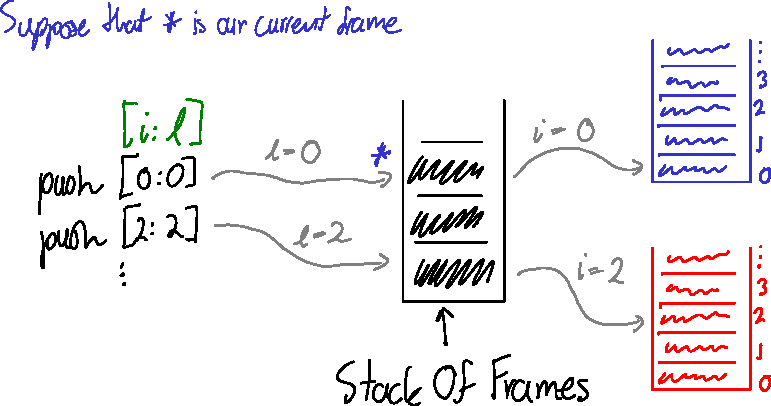
\includegraphics[width=\linewidth]{framesexp.pdf}
\end{mdframed}
\caption{A pictorial example of how the \mbox{\texttt{push
[i:l]}} operates.}
\label{fig:framesexp}
\end{figure}

\subsection{Properly Closing Scopes in Function Declarations}

A very important consideration when it comes to
function declarations is closing of scopes.

This is a problem of interest because functions should be
capable of returning anywhere within the body of a function even
if they are nested within multiple scopes.

\begin{lstlisting}[caption={A segment of the
\texttt{visit(Program *)} method in the \texttt{GenVisitor}
class (ir\_gen/GenVisitor.cpp).}, label=lst:framedepth]
...

emit_line("push {}", count);
emit_line("oframe");

mFrameDepth++;

...
\end{lstlisting}


\begin{lstlisting}[caption={The \texttt{visit(ReturnStmt *)}
method in the \texttt{GenVisitor} class
(ir\_gen/GenVisitor.cpp).}, label=lst:retstmt]
void GenVisitor::visit(core::ReturnStmt *stmt) {
    stmt->expr->accept(this);

    for (size_t i = 0; i < mFrameDepth; i++) {
        emit_line("cframe");
    }

    emit_line("ret");
}
\end{lstlisting}

To solve this issue, a variable \texttt{mFrameDepth} keeps track
of the number of frames open with the \texttt{oframe}
instruction, see \listref{framedepth}. When a return statement
node is reached the close frame instruction, \texttt{cframe}, is
emitted as many times as \\ \texttt{mFrameDepth} (see
\listref{retstmt}). This ensures that extra open frames are
closed before returning, allowing the VM to continue executing
the program normally.

\subsection{Assignments}

Similar, to when variables are first declared the store
(\texttt{st}) instruction is used for mutating the value in a
specified location. However, unlike variable declarations which
always define a level of $0$, assignments/mutations can occur on
variables defined in outer scopes. Hence, the level of variable
access needs to be calculated before being emitting \texttt{st}
and it necessary operands.

\begin{lstlisting}[caption={The \texttt{computeLevel()} method
in the \texttt{GenVisitor} class (ir\_gen/GenVisitor.cpp).},
label=lst:computelevel]
size_t GenVisitor::computeLevel(Environment *stoppingEnv) {
    size_t level = 0;

    Environment *env = mRefStack.currentEnv();

    while (stoppingEnv != env) {
        switch (env->getType()) {
            case Environment::Type::FOR:
            case Environment::Type::BLOCK:
                level++;
                break;
            case Environment::Type::FUNCTION:
                core::abort("unreachable");
                break;
            default:
                // noop
                break;
        }

        env = env->getEnclosing();
    }

    return level;
}
\end{lstlisting}

The basic idea for calculating the level of a variable is as
follows, copy the pointer to the \texttt{Environment} which
holds the variable then traverse from the current
\texttt{Environment} until the \texttt{Environment} with the
exact pointer as the \texttt{Environment} the variable was found
in is reached, all the while keeping track of the number of
scopes jumped through to reach said environment.

\begin{note}
Not, all \texttt{Environment}s contribute an open frame
(\texttt{oframe}), hence only certain types of scopes should be
counted as contributing to the number of levels. In the case of
\texttt{PArL} with its current restrictions, the only such
scopes are for-scopes and block-scopes (see
\listref{computelevel}).
\end{note}

\subsection{Expressions}

\subsubsection{Type Specific VM Code}

\begin{lstlisting}[caption={A segment of the
\texttt{visit(Binary *)} method in the \texttt{GenVisitor} class
(ir\_gen/GenVisitor.cpp).}, label=lst:overloadeddiv]
...
case core::Operation::DIV: {
    core::Primitive type = mType.getType(
        expr->right.get(),
        mRefStack.getGlobal(),
        mRefStack.currentEnv()
    );
    if (type == core::Primitive{core::Base::INT}) {
        expr->right->accept(this);
        expr->right->accept(this);
        expr->left->accept(this);
        emit_line("mod");
        expr->left->accept(this);
        emit_line("sub");
        emit_line("div");
    } else {
        expr->right->accept(this);
        expr->left->accept(this);
        emit_line("div");
    }
} break;
...
\end{lstlisting}

When it comes to expressions, due to the fact that operators
within the \texttt{PArL} language are overloaded some attention
to detail is required. The majority of the usage of
\texttt{TypeVisitor} is within expression nodes, specifically,
in places where behaviour is dependent on the operand's types.
For example in the case of division, the type of one of the
operands is computed (recall that semantic analysis guarantees
consistency of types, in the case of binary operations both the
left and right operands have the same type), then different
instructions are emitted depending on the returned type (see
\listref{overloadeddiv}).

\subsubsection{Function Calls}

\begin{lstlisting}[caption={The \texttt{visit(FunctionCall *)}
method in the \texttt{GenVisitor} class
(ir\_gen/GenVisitor.cpp).}, label=lst:funccall]
void GenVisitor::visit(core::FunctionCall *expr) {
    for (auto itr = expr->params.rbegin();
         itr != expr->params.rend();
         itr++) {
        (*itr)->accept(this);
    }

    size_t size{0};

    for (auto &param : expr->params) {
        core::Primitive paramType = mType.getType(
            param.get(),
            mRefStack.getGlobal(),
            mRefStack.currentEnv()
        );

        size += paramType.is<core::Array>()
                    ? paramType.as<core::Array>().size
                    : 1;
    }

    emit_line("push {}", size);
    emit_line("push .{}", expr->identifier);
    emit_line("call");
}
\end{lstlisting}

Functions calls are performed using the \texttt{call} VM
instruction. The most important aspect of function calls,
similar to scopes, is the calculation of the total size of the
parameters. This essentially determines how many operands will
be popped of off the operand stack and moved into the implicitly
created function frame. Additionally, it is important for all
the parameters of a function to be evaluated in reverse order
due to the fact that popping from the operand stack into the
function frame reverse the order of the parameters (see
\listref{funccall}).

\subsection{Branching}

Branching is somewhat challenging since at the jumping point the
compiler is unaware of how many instructions it might need to
jump. There are two possible solutions for this problem. The
first is to create a visitor which is capable of calculating the
number of instruction which a node expands to. The second makes
use of a placeholder instruction that is then changed after the
rest of the associated instructions are generated.

Previous iterations of the \texttt{PArL} compiler used the first
approach however, the first approach is quite unmaintainable
since changes in other areas of the code generation would
require changes in the visitor which computes the number of
instructions. Hence, the compiler was changed to adopt the
second approach.

\texttt{PArL} has only three node types which branch, if-else
statements, for-loops and while-loops.

\begin{lstlisting}[caption={The \texttt{visit(WhileStmt *)}
method in the \texttt{GenVisitor} class
(ir\_gen/GenVisitor.cpp).}, label=lst:whilestmtgen]
void GenVisitor::visit(core::WhileStmt *stmt) {
    mRefStack.pushEnv();

    size_t condOffset = PC();

    stmt->cond->accept(this);

    emit_line("not");

    size_t patchOffset = PC();

    emit_line("push #PC+{{}}");
    emit_line("cjmp");

    stmt->block->accept(this);

    emit_line("push #PC-{}", PC() - condOffset);
    emit_line("jmp");

    mCode[patchOffset] =
        fmt::format(mCode[patchOffset], PC() - patchOffset);

    mRefStack.popEnv();
}
\end{lstlisting}

Both for-loops and while-loops branch in the same manner.
Patching the relevant instructions for branching in for- and
while-loops works as follows (additionally, see
\listref{whilestmtgen}):

\begin{enumerate}
    \item The location of the instruction which starts the
        condition is stored (in this case in
        \texttt{condOffset});
    \item the location of the `\texttt{push \#PC+\{\}}'
        instruction used for \texttt{cjmp} is stored (in this
        case in \texttt{patchOffset});
    \item then the block associated with the for- or while-loop
        accepts the \texttt{GenVisitor}, emitting further
        instructions;
    \item the offset required to jump back to the
        start of the condition instructions is calculated and
        used with a \texttt{jmp} instruction;
    \item and finally, the `\texttt{push \#PC+\{\}}' instruction
        at \texttt{patchOffset} is patched with the appropriate
        offset to jump clear all of the for- or while- loop
        instructions.
\end{enumerate}

\begin{lstlisting}[caption={The \texttt{visit(IfStmt *)} method
in the \texttt{GenVisitor} class (ir\_gen/GenVisitor.cpp).},
label=lst:ifstmtgen]
void GenVisitor::visit(core::IfStmt *stmt) {
    if (stmt->elseBlock) {
        mRefStack.pushEnv();

        stmt->cond->accept(this);

        emit_line("not");

        size_t ifPatchOffset = PC();

        emit_line("push #PC+{{}}");
        emit_line("cjmp");

        stmt->thenBlock->accept(this);

        mRefStack.popEnv();

        mRefStack.pushEnv();

        size_t elsePatchOffset = PC();

        emit_line("push #PC+{{}}");
        emit_line("jmp");

        mCode[ifPatchOffset] = fmt::format(
            mCode[ifPatchOffset],
            PC() - ifPatchOffset
        );

        stmt->elseBlock->accept(this);

        mCode[elsePatchOffset] = fmt::format(
            mCode[elsePatchOffset],
            PC() - elsePatchOffset
        );

        mRefStack.popEnv();
    } else {
        mRefStack.pushEnv();

        stmt->cond->accept(this);

        emit_line("not");

        size_t patchOffset = PC();

        emit_line("push #PC+{{}}");
        emit_line("cjmp");

        stmt->thenBlock->accept(this);

        mCode[patchOffset] = fmt::format(
            mCode[patchOffset],
            PC() - patchOffset
        );

        mRefStack.popEnv();
    }
}
\end{lstlisting}

The other form of branching, if-else statements, is a bit more
involved. This is because there are two cases which need
consideration: when only an \texttt{if} is present and when both
an \texttt{if} and an \texttt{else} are present. Nevertheless,
the basic principal is the same, offsets into the code are used
and specific lines are patched after (see \listref{ifstmtgen}).

\section{Arrays}

Adding support for arrays in \texttt{PArL} had driven a number
of changes across the whole of the compiler. Some of the changes
will be explained in the following sections whilst others where
already described in earlier sections due to the fundamental
changes they caused.

\subsection{Changes in Lexical Analysis}

\begin{lstlisting}[caption={Changes in the
\texttt{LexerDirector} for supporting left (`\texttt{[}') and
right (`\texttt{]}') brackets (lexer/LexerDirector.cpp).}]
...

.addCategory(
    LEFT_BRACKET,
    [](char c) -> bool {
        return c == '[';
    }
)
.addCategory(
    RIGHT_BRACKET,
    [](char c) -> bool {
        return c == ']';
    }
)

...

.addTransition(0, LEFT_BRACKET, 20)
.addTransition(0, RIGHT_BRACKET, 21)

...

.setStateAsFinal(20, Token::Type::LEFT_BRACK)
.setStateAsFinal(21, Token::Type::RIGHT_BRACK)

...
\end{lstlisting}


Within lexical analysis a very lax approach to arrays was
adopted that is, there is no enforcement of the more complicated
$\langle$Identifier$\rangle$ syntax proposed in the original
EBNF of the language. The only additions have been support for
consuming left (`\texttt{[}') and right (`\texttt{]}') brackets.

\subsection{Changes in Parsing}

As described in \ref{sss:secarrays}, the grammar of the language
was significantly reordered to improve the upgrade-ability of
the language down the line. Additionally, the majority of the
changes to the parser where also discussed in
\ref{sss:secarrays}.

\begin{todo}
The addition of de-sugaring, type inference and more types is
facilitated by the changes proposed in the EBNF. These additions
would allow for more complicated language mechanisms and hence
an improved developer experience.
\end{todo}

\subsection{Changes in Semantic Analysis}

Again due to the changes in the way types are managed (again see
\ref{sss:primitive}), the following notable changes where
required: extra validation, restriction on type casting,
figuring out the type of array access and finally, generating
the type for array literals.

\begin{lstlisting}[caption={A part of the \texttt{visit(Binary
*)} method in the \texttt{AnalysisVisitor} class
(analysis/AnalysisVisitor.cpp).}]
...
case core::Operation::ADD:
case core::Operation::SUB:
    if (leftType.is<core::Array>()) {
        error(
            expr->position,
            "operator {} is not defined on array "
            "types",
            core::operationToString(expr->op)
        );
    }

    if (leftType != rightType) {
        error(
            expr->position,
            "operator {} expects both operands to "
            "be of same type",
            core::operationToString(expr->op)
        );
    }

    mReturn = leftType;
    break;
...
\end{lstlisting}

Of course, validation is necessary to ensure that arrays do no
interact with each other, for example \texttt{[1,2,3] + [1,2,3]}
is not semantically correct in \texttt{PArL}.

\begin{lstlisting}[caption={The \texttt{isViableCast()} method
in the \texttt{AnalysisVisitor} class
(analysis/AnalysisVisitor.cpp).}]
void AnalysisVisitor::isViableCast(
    core::Primitive &from,
    core::Primitive &to

) {
    const core::Primitive *lPtr = &from;
    const core::Primitive *rPtr = &to;

    while (lPtr != nullptr && rPtr != nullptr) {
        if (lPtr->is<core::Base>() &&
            rPtr->is<core::Array>()) {
            error(
                mPosition,
                "primitive cannot be cast to an array"
            );
        }

        if (lPtr->is<core::Array>() &&
            rPtr->is<core::Base>()) {
            error(
                mPosition,
                "array cannot be cast to a primitive"
            );
        }

        if (lPtr->is<core::Array>() &&
            rPtr->is<core::Array>()) {
            size_t lSize = lPtr->as<core::Array>().size;
            size_t rSize = rPtr->as<core::Array>().size;

            lPtr = lPtr->as<core::Array>().type.get();
            rPtr = rPtr->as<core::Array>().type.get();

            if (lSize != rSize) {
                error(
                    mPosition,
                    "array of size {} cannot be cast to an "
                    "array of size {}",
                    lSize,
                    rSize
                );
            }

            continue;
        }

        return;
    }

    core::abort("unreachable");
}
\end{lstlisting}

Necessary checks to ensure that casting is viable, needed to be
considered. This approach was taken over allowing all forms of
casting because casting from one type to another where the sizes
of the types are different would result in substantial
complexity later on in code generation.

Consider the following example:

\begin{center}
\begin{minipage}[l]{0.54\linewidth}
\begin{lstlisting}[morekeywords={color}]
let x: int[5] = [1,2,3,4,5];
let y: int = (x as color[10])[6];
\end{lstlisting}
\end{minipage}
\end{center}

Not only is there ambiguity as to what the upper elements of the
type cast should be but additional padding is necessary to
ensure no out of of bounds accesses during VM execution.

Finally, the process of computing the type of an array access
and an array literal is quite easy, see
analysis/AnalysisVisitor.cpp lines 252 and 170 respectively.

\subsection{Changes in Code Generation}

One of the more important changes for code generation is the
calculation of frame sizes. This has already been described in
detail even in the context of arrays in the note in
\ref{sss:framesizecalc}. Of course where appropriate
\texttt{sta}, \texttt{pusha}, \texttt{printa} and \texttt{push
+[i:l]} which are meant for storing arrays, pushing arrays onto
the operand stack, printing arrays and pushing an single element
of an array onto the operand stack respectively, are being used
accordingly. See ir\_gen/GenVisitor.cpp, lines 456, 111, 478 and
166, for examples of each.

A decision to opt out of using \texttt{reta} was made due to the
inconsistent behaviour of arrays in the VM. Instead a hack for
reversing the order manually was devised.

\begin{lstlisting}[caption={A part of the \texttt{visit(Variable
*)} method in the \texttt{GenVisitor} class, specifically the
hack mentioned above (ir\_gen/GenVisitor.cpp).},label=lst:hack]
...
if (symbol.type.is<core::Array>()) {
    size_t arraySize =
        symbol.type.as<core::Array>().size;
    emit_line("push {}", arraySize);
    emit_line("pusha [{}:{}]", symbol.idx, level);
    emit_line("push {} // START HACK", arraySize);
    emit_line("oframe");
    emit_line("push {}", arraySize);
    emit_line("push 0");
    emit_line("push 0");
    emit_line("sta");
    emit_line("push {}", arraySize);
    emit_line("pusha [0:0]");
    emit_line("cframe // END HACK");

    return;
}
...
\end{lstlisting}

The problem of arrays is the following:

Consider the following code: \texttt{\_\_print [1,2,3];}

\begin{center}
\begin{tabular}{c}
\begin{lstlisting}[morekeywords={push, printa, oframe, cframe,
halt},frame=none]
  .main
  push 0
  oframe
  push 3
  push 2
  push 1
  push 3
  printa
  cframe
  halt
\end{lstlisting}
\end{tabular}
\end{center}

It generates the code above and what is important to
notice is the last element in the array is the first to be
pushed onto the operand stack ensuring that printing is correct.

However, now consider the following piece of code: \texttt{let
x: int[3] = [1,2,3]; \_\_print x;}

\begin{center}
\begin{tabular}{c}
\begin{lstlisting}[morekeywords={sta, push, pusha, printa, oframe,
cframe, halt},frame=none]
  .main
  push 3
  oframe
  push 3
  push 2
  push 1
  push 3
  push 0
  push 0
  sta
  push 3
  pusha [0:0]
  push 3
  printa
  cframe
  halt
\end{lstlisting}
\end{tabular}
\end{center}

The naïve implementation generates the code on the left. Running
this on the VM one would expect the exact same output as the
first. However, this is not the case the order of the elements
is reversed.

\begin{figure}[H]
    \centering
    \begin{framefig}
    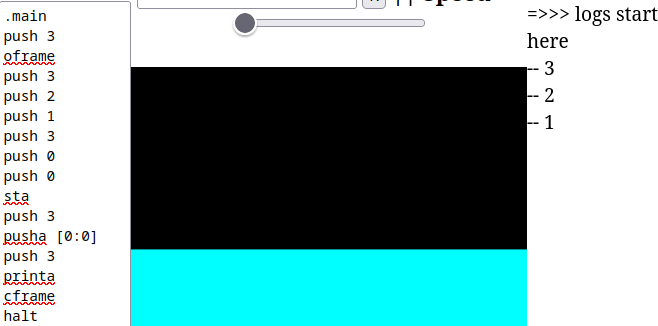
\includegraphics[width=0.95\linewidth]{naivepusha.png}
    \end{framefig}
    \caption{The result of running the code generated by
    \texttt{let x: int[3] = [1,2,3]; \_\_print x;} in the VM.}
\end{figure}

This happens because reading from a frame using \texttt{pusha}
actually reverse the order of the elements on the operand stack.
To circumvent this issue a second temporary frame is created
where the elements are stored in the frame and read again
reversing the order one-more time into the correct order (see
\listref{hack}).

Due to this hack which works in all situations \texttt{reta} is
not being used as it would flip the order again.

\section{Testing \& Usage}

\subsection{Usage}

The current produced binary accepts the following flags
\texttt{-d}, \texttt{-l}, \texttt{-p}. \texttt{-d} is currently
disabled, \texttt{-l} prints each of the lexemes generated by
the source and \texttt{-p} outputs the AST both before and after
preprocessing.

\subsection{The Lexer, Parser \& Semantic Analyser}

As discussed in previous sections all the phases which are
capable of producing errors or warnings are either doing so
manually using \texttt{fmt::println(stderr, ...)} or using some
customised methods like \texttt{error(...)} or
\texttt{warning(...)}. Additionally, as described in previous
sections as well, the lexer, parser and analyser should not fail
upon the first inconsistency within the program, instead they
should proceed to a state in which they continue processing
normally.

The main aim of testing will be to make sure that both correct
and incorrect input produce the expected behaviour.

\subsubsection{Lexical Analysis}

\begin{figure}[H]
\centering
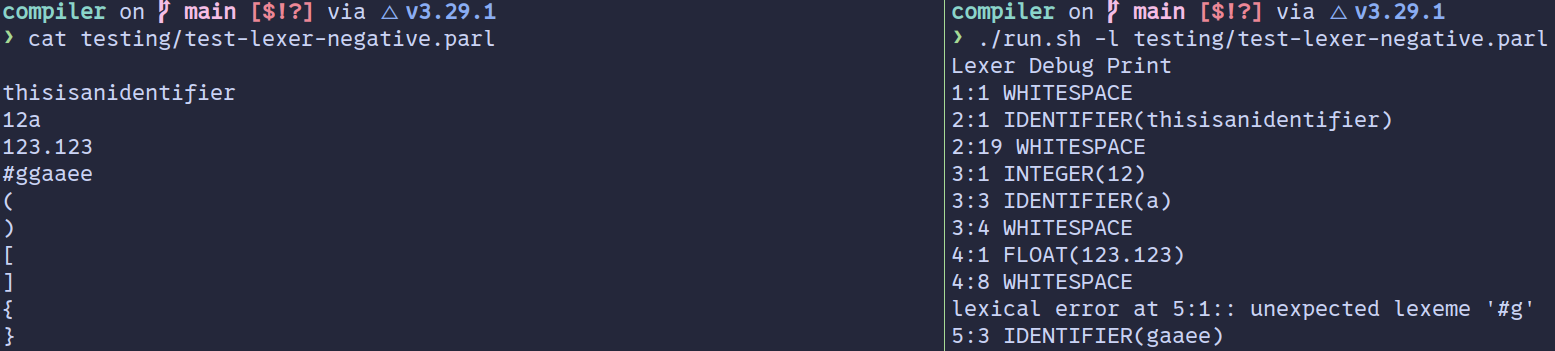
\includegraphics[width=\linewidth]{lexernegative.png}
\caption{Running the negative lexer test
(testing/test-lexer-negative.parl)}
\end{figure}

For lexical analysis two major tests where used,
testing/test-lexer-negative.parl and
testing/test-lexer-positive.parl. Additional, tests include,
testing/test1.parl upto testing/test9.parl.

\subsubsection{Parsing}

\begin{figure}[H]
\centering
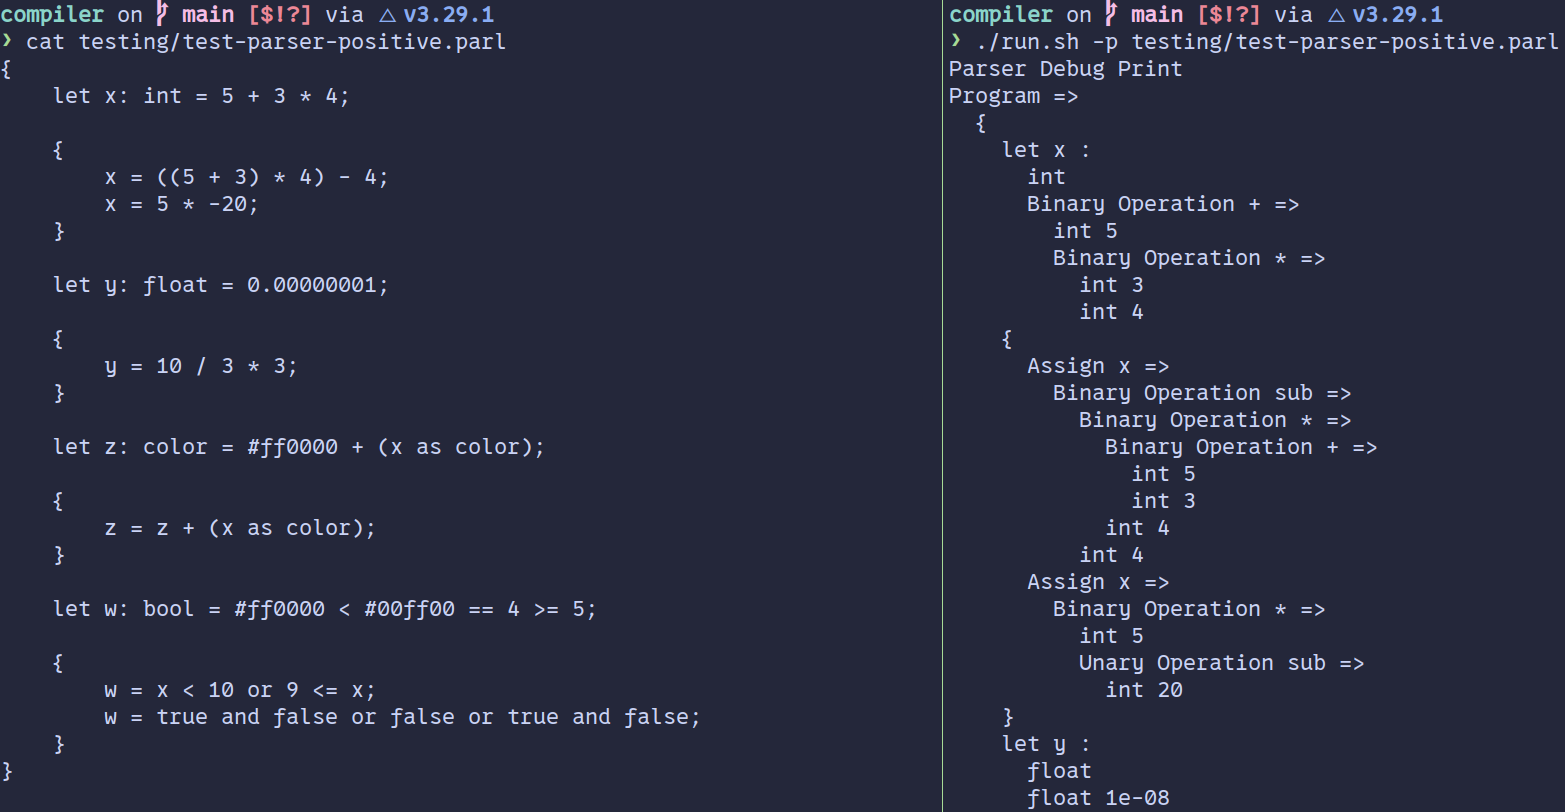
\includegraphics[width=\linewidth]{parserpositive.png}
\caption{Running the positive parser test
(testing/test-parser-positive.parl)}
\end{figure}

Again for parsing two major tests where developed
testing/test-parser-negative.parl and
testing/test-parser-positive.parl.

\begin{figure}[H]
\centering
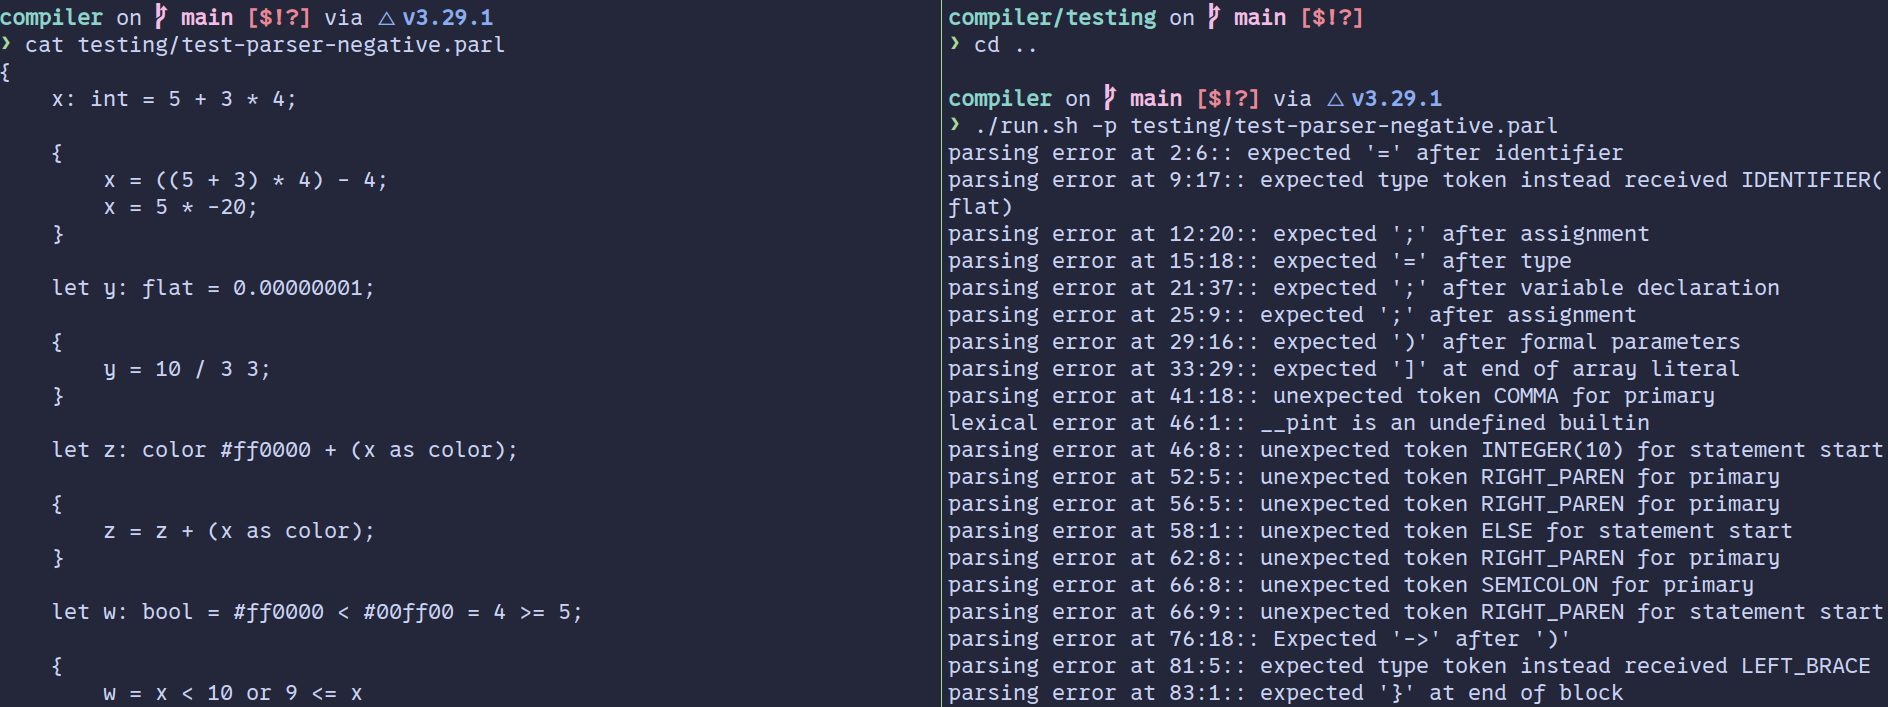
\includegraphics[width=\linewidth]{parsernegative.png}
\caption{Running the negative parser test
(testing/test-parser-negative.parl)}
\end{figure}

In particular the positive test covers of the happy paths of the
parser. However, there are way more possibilities where the
parser flags the input as not conforming to the grammar. Hence,
not all possible code paths are being tested with the negative
test. Additional, files used for testing during development
include: testing/test10.parl, testing/test15.parl and
testing/test16.parl.

\subsubsection{Semantic Analysis}

\begin{figure}[H]
\centering
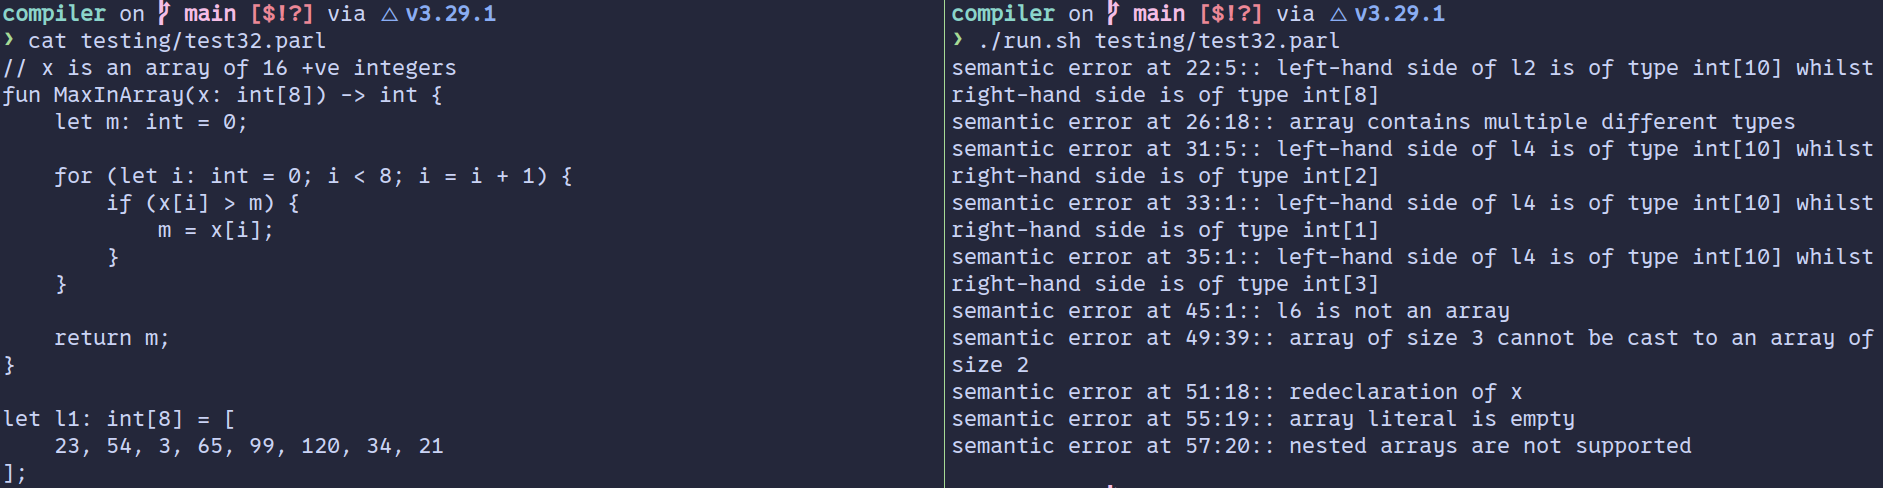
\includegraphics[width=\linewidth]{test32.png}
\caption{Running test 32 (testing/test32.parl)}
\end{figure}

Semantic analysis is again a leap in complexity. And hence, the
order of possible errors and issues is also greater. Because of
this completely testing all possible scenarios is very diffcult.
Instead the tests presented and mentioned are those written
during development to test certain aspects of the semantic
analyser as it was being developed.

The tests mentioned above are:

\begin{itemize}
    \item testing/test13.parl;
    \item testing/test14.parl;
    \item testing/test17.parl;
    \item testing/test18.parl (parameter types);
    \item testing/test19.parl (parameter types);
    \item testing/test21.parl (casting);
    \item testing/test23.parl (no main functions);
    \item testing/test24.parl (for nested functions);
    \item testing/test25.parl;
    \item testing/test28.parl (for unreachable code);
    \item testing/test31.parl (for arrays);
    \item testing/test32.parl;
    \item testing/test33.parl;
    \item testing/test41.parl (for unreachable code).
    \item testing/test41.parl (for unreachable code).
    \item testing/test45.parl (recursive call chain).
\end{itemize}

Some additional, tests have been run during the recording at,
\url{https://drive.google.com/file/d/11HW-MxJbIX9eFRX1wTw9koo4Rzl0bTND/view?usp=sharing}.

\subsection{Code Generation}

\begin{figure}[H]
\centering
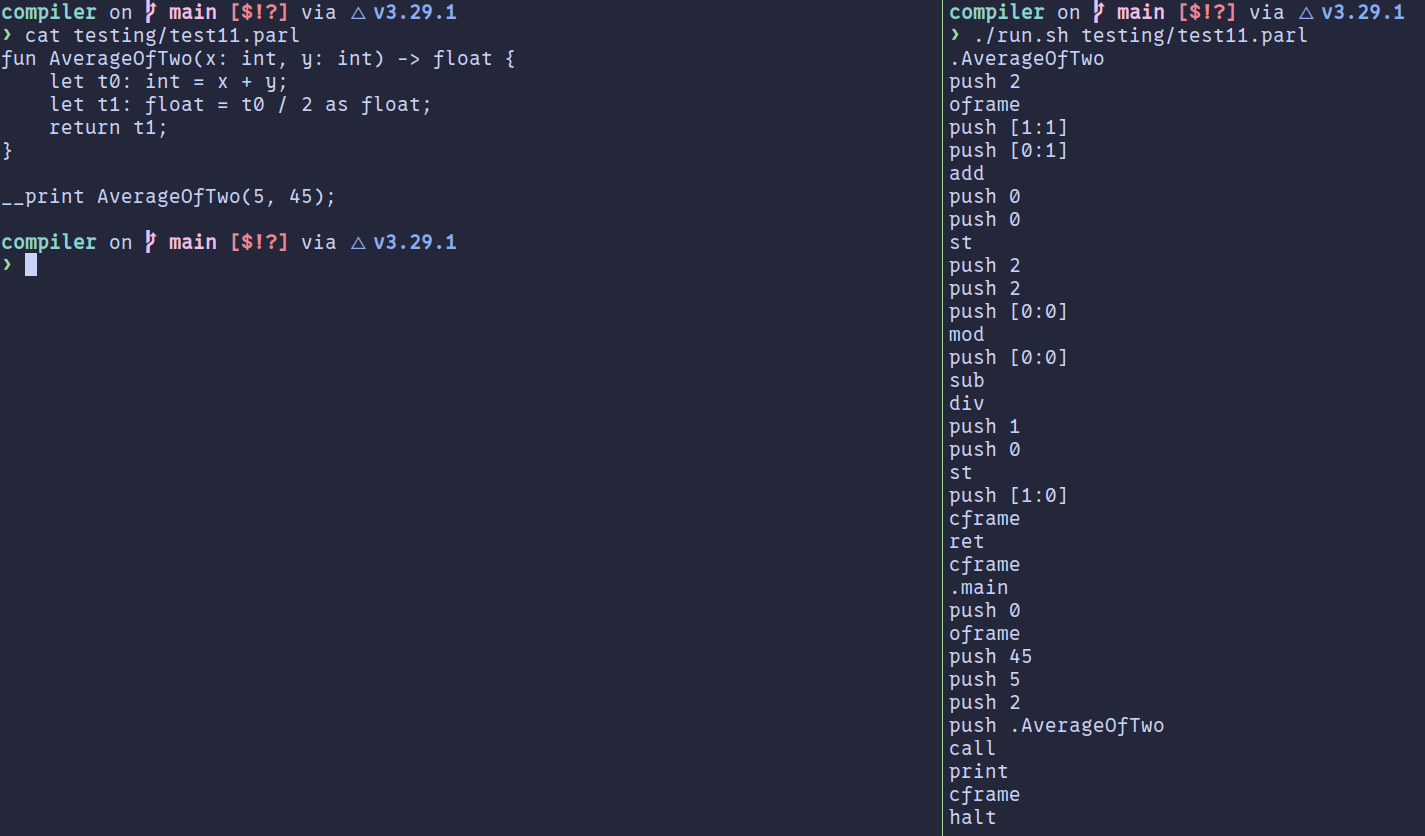
\includegraphics[width=\linewidth]{test11.png}
\caption{Running test 11 (testing/test11.parl)}
\end{figure}

Code generation was tested using a number of semantically valid
programs. The following is a list of such programs:

\begin{itemize}
    \item testing/test11.parl
    \item testing/test20.parl
    \item testing/test26.parl
    \item testing/test27.parl
    \item testing/test29.parl
    \item testing/test30.parl
    \item testing/test34.parl
    \item testing/test37.parl
    \item testing/test45.parl
\end{itemize}

Again, some additional examples are run in the video at
\url{https://drive.google.com/file/d/11HW-MxJbIX9eFRX1wTw9koo4Rzl0bTND/view?usp=sharing}.

\subsection{Video}

The video is a the usage of the compiler with a selection of a
few hand-picked examples, in particular: test30.parl,
test37.parl, test41.parl and test45.parl.

The video can be view at the following URL:
\url{https://drive.google.com/file/d/11HW-MxJbIX9eFRX1wTw9koo4Rzl0bTND/view?usp=sharing}.

\section{Limitations}

The only known limitations of the compiler in relation to the
specification is the lack of sytanx sugar for the array syntax
as described in \ref{eyecandy}.


\end{document}
